\documentclass[compress]{beamer}

\usetheme{Szeged}
\RequirePackage[T1]{fontenc}
\RequirePackage[utf8]{inputenc}
\RequirePackage[frenchb]{babel}
\usepackage[babel=true,kerning=true]{microtype}
\usepackage{tikz,listings,algorithm,algorithmic}
\usetikzlibrary{automata,shapes,snakes,arrows}

\tikzstyle{every picture}=[sibling distance=3cm, shorten >=1pt, node distance=2cm,%
	>=stealth', bend angle=10, auto, initial text=]

\title[SEM IN310 - Réseaux de Petri]{Réseaux de Petri\\IN310 - Modèles des SE}
\author[Charles Lesire]{Charles Lesire-Cabaniols (ONERA / DCSD)\\{\tt charles.lesire@onera.fr}}
\date[2010-2011]{3A-SEM - 2010-2011}

\graphicspath{{../figures/}}
\lstset{basicstyle=\tiny,tabsize=2,
	emph={define,domain,requirements,strips,typing,types,predicates,
		action,parameters,precondition,vars,effect,objects,init,goal},%
	emphstyle=\bf}

\begin{document}

\begin{frame}
\titlepage
\end{frame}

\begin{frame}
\tableofcontents[hidesubsections]
\end{frame}

\section{Introduction}
\subsection{Introduction}
\begin{frame}{Introduction}
\begin{itemize}
\item 1962, Carl Adam Petri: Communication et composition entre automates
\item Outil de modélisation de systèmes dynamiques : permet de raisonner sur les objets, les ressources et leur changement d'état
\item Outil mathématique (formel) et outil graphique
	\begin{itemize}
	\item permet de représenter le vrai parallélisme, la concurrence, contraintes de précédence,
	\item analyse de bonnes propriétés (vivacité, borné, etc.) et propriétés structurelles : aide efficiente durant les phases de conception
	\item peut être simulé et implémenté directement par un joueur de RdP
	\end{itemize} 
\end{itemize} 
\end{frame}

\begin{frame}{Introduction}
\begin{itemize}
\item Applications:
	\begin{itemize}
	\item évaluation de performances, 
	\item analyse et vérification formelles, 
	\item protocoles de communication, 
	\item contrôle de systèmes de production, 
	\item systèmes d'information (organisation d'entreprises), 
	\item gestion de bases de données, 
	\item IHM, etc.
	\end{itemize} 
\end{itemize} 
\end{frame}

\begin{frame}{Introduction}
\begin{itemize}
\item Etat : les différentes {\it phases} par lesquelles passe le système;
\item Variables d'état : ensemble de variables qui permettent de connaître l'état du système.
	\begin{itemize}
	\item Système continu : les variables d'état évoluent continuellement dans le temps;
	\item Système à événements discrets : les variables d'état changent {\it brusquement} à certains instants
	\end{itemize}
\item Evénement : son occurrence fait changer l'état du système
\item Activité : {\it boîte noire} représente lŽévolution du système entre 2 événements
\item Processus : séquence dŽévénements et d'activités \\
	$\leadsto$  coopération, compétition, parallèle
\end{itemize}
\end{frame}

\subsection{Présentation informelle}     
\begin{frame}{Présentation informelle}
\begin{block}{Éléments de base}
\begin{itemize}
\item \structure{Place :} interprétée comme condition, état partiel, ensemble de ressources
\item \structure{Transition :} associée à un événement qui a lieu dans le système
\item \structure{Jeton :} indique que la condition associée à la place est vérifiée (ou le nombre d'éléments qui la vérifient)
\end{itemize}
\end{block}
\end{frame}

\begin{frame}{Présentation informelle}
\begin{block}{Comportement dynamique}
\begin{columns}
	\begin{column}{.7\textwidth}
	\begin{itemize}
	\item état : répartition des jetons dans les places,
	\item occurrence d'un événement : tir de la transition,
		\begin{itemize}
		\item  enlever les jetons des places d'entrée,
		\item  mettre les jetons dans les places de sortie.
		\end{itemize}
	\end{itemize}
	\end{column}	
	\begin{column}{.3\textwidth}
		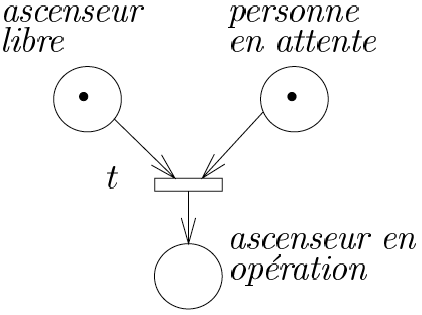
\includegraphics[width=3.2cm]{frdp}
	\end{column}
\end{columns}
\end{block}
\end{frame}

\section{Modèle formel}
\subsection{Définition}
\begin{frame}{Définitions}
\begin{itemize}
\item Modèle formel, peut être caractérisé par :
	\begin{itemize}
	\item graphe avec comportement dynamique ; représentation naturelle pour le concepteur,
	\item ensemble de matrices d'entiers : comportement dynamique décrit par un système linéaire :  représentation naturel pour l'ordinateur ;
	\item système de règles: peut être utilisé avec les techniques d'I.A;
	\end{itemize}     
\item Validation par analyse et simulation ;
\item Représente: parallélisme, synchronisme, séquence, conflit, concurrence.
\end{itemize}
\end{frame}
 
\begin{frame}{Définitions}
\begin{block}{Réseaux de Petri $R = <\!P, T, Pre, Post\!>$}
	\begin{itemize}
	\item $P$ est un ensemble fini de places de dimension $n$;
	\item $T$ est un ensemble fini de transitions de dimension $m$;
	\item $Pre : P \times T \rightarrow \mathbb{N}$ est l'application d'{\it entrée} (places précédentes),
	\item $Post:P \times T \rightarrow \mathbb{N}$ est l'application de {\it sortie} (places suivantes),
	\end{itemize}
\end{block}
\begin{block}{Réseau de Petri marqué $N = <\!R,M\!>$}
	\begin{itemize}
	\item $R$ est un réseau de Petri,
	\item $M : P \rightarrow \mathbb{N}$ est le marquage initial \\
		(distribution de jetons dans les places)
	\end{itemize}
\end{block}
\end{frame}

\begin{frame}{Définitions}
\begin{block}{Exemple}
\begin{columns}
	\begin{column}{.7\textwidth}
		\begin{itemize}
		\item $R = <\!P, T, Pre, Post\!>$\\
		\item $P=\{p_1,p_2,p_3\}$
		\item $T=\{a,b,c,d\}$
		\item $Post(p_1,a)=1$, $Pre(p_1,b)=1$, $Post(p_2,b)=1$
		\end{itemize}
	\end{column}
	\begin{column}{.3\textwidth}
		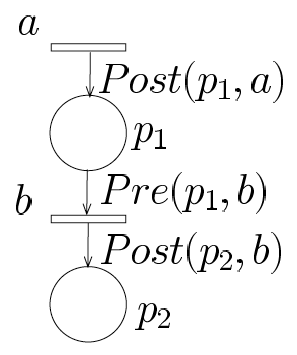
\includegraphics[width=2.8cm]{pre}
	\end{column}	
\end{columns}
\end{block}
\end{frame}

\begin{frame}{Graphe et notation matricielle}
\begin{block}{Réseau de Petri marqué $N=<\!R,M\!>$}
\begin{columns}
	\begin{column}{.5\textwidth}
		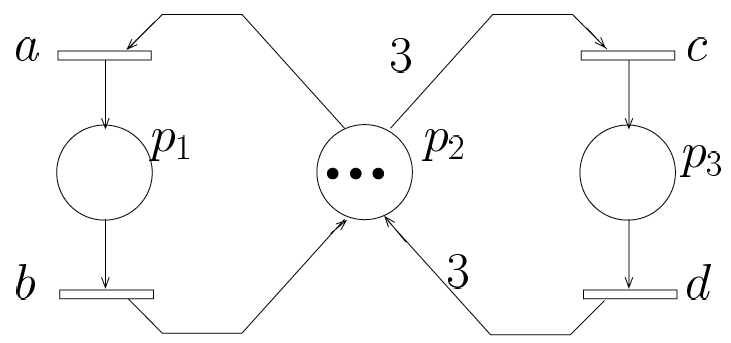
\includegraphics[width=5.5cm]{lececr}
	\end{column}
	\begin{column}{.6\textwidth}
		$$P=\{p_1,p_2,p_3\}, \qquad T=\{a,b,c,d\}$$
		$$Pre = \begin{pmatrix}
			0 & 1 & 0 & 0 \\
			1 & 0 & 3 & 0 \\
			0 & 0 & 0 & 1 
			\end{pmatrix}$$
		$$Post = \begin{pmatrix}
			1 & 0 & 0 & 0 \\
			0 & 1 & 0 & 3 \\
			0 & 0 & 1 & 0 
			\end{pmatrix}$$
		$${}^tM = \begin{pmatrix}0 & 3 & 0\end{pmatrix}$$
	\end{column}	
\end{columns}
\end{block}
\end{frame}

\subsection{Structures}
\begin{frame}{Différentes interactions entre les processus}
\begin{block}{Séquence}
	\begin{center}
		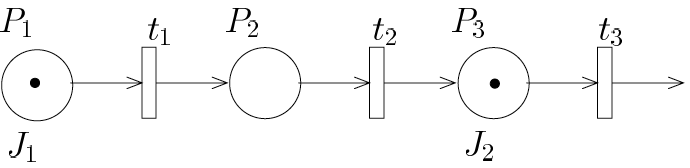
\includegraphics[width=.6\linewidth]{fseq-inf}
	\end{center}
	\begin{itemize}
	\item séquence d'un processus de fabrication :
	   \begin{itemize}
	   \item $P_i$ : phase $i$ de l'opération sur la pièce, 
	   \item $t_i$ : passage d'une phase à une autre;
	   \end{itemize}
	\item portion de l'itinéraire d'un système de transport :     
	   \begin{itemize}
	   \item $P_i$ : chariot traverse la section $i$,
	   \item $t_i$ : passage d'un chariot d'une section  à une autre;
	   \end{itemize}
	\end{itemize}
%$\leadsto$ deux systèmes {\it différents}, mais avec un comportement analogue,
%possèdent le {\it même} modèle de RdP!
\end{block}
\end{frame}
 
\begin{frame}{Différentes interactions entre les processus}
\begin{block}{Fork}
\begin{columns}
	\begin{column}{.3\linewidth}
		\begin{center}
			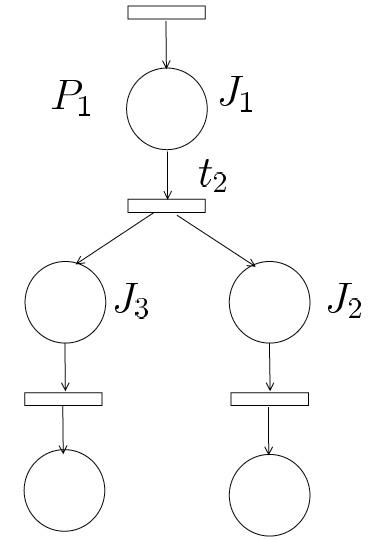
\includegraphics[width=\linewidth]{div}
		\end{center}
	\end{column}
	\begin{column}{.7\linewidth}
		\begin{itemize}
		\item à partir de l'activité $J_1$, deux activités sont crées ($J_2$ et $J_3$),
		\item $J_2$ et  $J_3$ évoluent de façon indépendante.
		\end{itemize} 
	\end{column}
\end{columns}
\end{block}
\end{frame}

\begin{frame}{Différentes interactions entre les processus}
\begin{block}{Join}
\begin{columns}
	\begin{column}{.3\linewidth}
		\begin{center}
			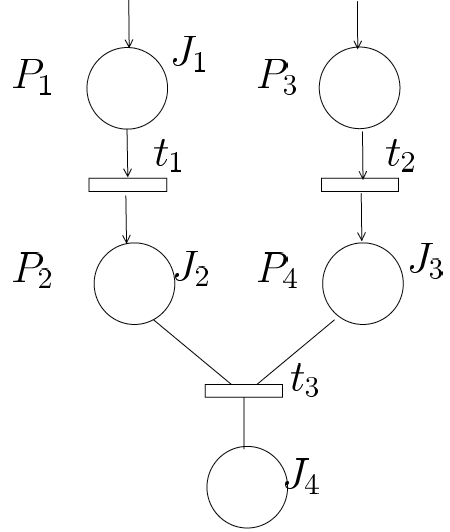
\includegraphics[width=\linewidth]{jun}
		\end{center}
	\end{column}
	\begin{column}{.7\linewidth}
		\begin{itemize}
		\item évolution indépendante de $t_1$ et $t_2$ (évolution assynchrone),
		\item synchronisme en $t_3$.
		\end{itemize}
	\end{column}
\end{columns}
\end{block}
\end{frame}

\begin{frame}{Différentes interactions entre les processus}
\begin{block}{Choix}
\begin{columns}
	\begin{column}{.3\linewidth}
		\begin{center}
			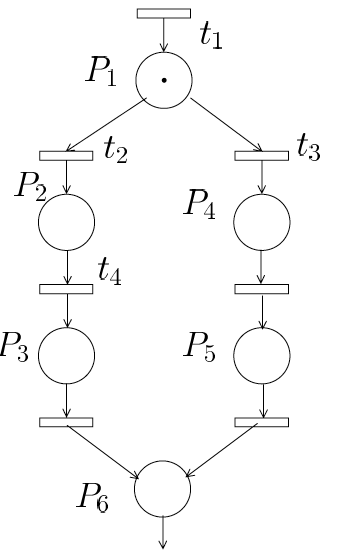
\includegraphics[width=\linewidth]{alt}
		\end{center}
	\end{column}
	\begin{column}{.7\linewidth}
		\begin{itemize}
		\item choix entre $t_2$ (seq. $P_2P_3$) et $t_3$ (seq. $P_4P_5$): seulement une peut être tirée;
		\item les 2 séquences exécuteront $P_6$.
		\end{itemize} 
	\end{column}
\end{columns}
\end{block}
\end{frame}

\begin{frame}{Différentes interactions entre les processus}
\begin{block}{Répétition}
\begin{columns}
	\begin{column}{.3\linewidth}
		\begin{center}
			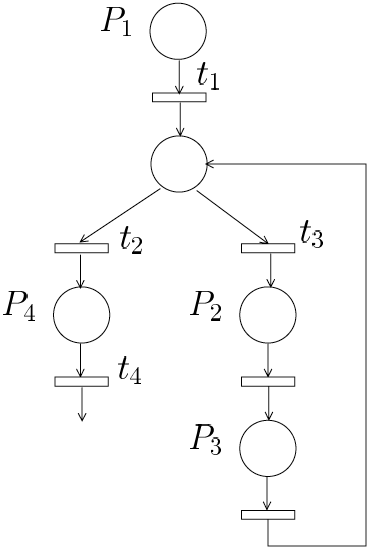
\includegraphics[width=\linewidth]{rep}
		\end{center}
	\end{column}
	\begin{column}{.7\linewidth}
		\begin{itemize}
		\item choix entre $t_2$ e $t_3$,
		\item répéter la séq. $P_2P_3$ un certain nombre de fois avant de exécuter $P_4$.
		\end{itemize}
	\end{column}
\end{columns}
\end{block}
\end{frame}

\begin{frame}{Différentes interactions entre les processus}
\begin{block}{Allocation de ressources}
\begin{columns}
	\begin{column}{.3\linewidth}
		\begin{center}
			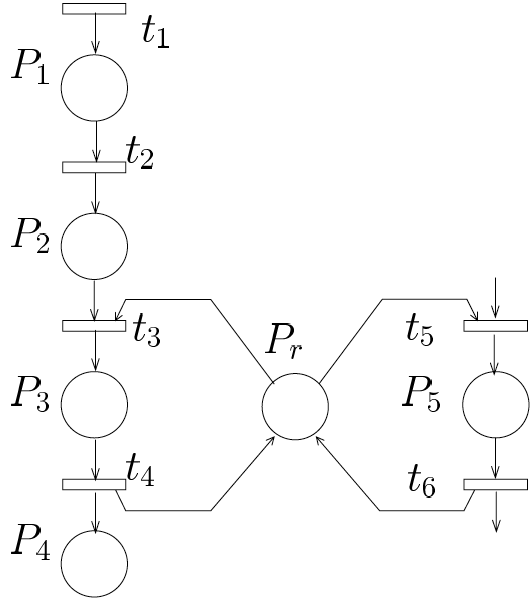
\includegraphics[width=\linewidth]{frecurso}
		\end{center}
	\end{column}
	\begin{column}{.7\linewidth}
		\begin{itemize}
		\item un même chariot doit servir différentes machines,
		\item un opérateur doit exécuter  différentes activités (une à la fois).
		\end{itemize}  
	\end{column}
\end{columns}
\end{block}
\end{frame}

\begin{frame}{Exemple : Système par lot}
\begin{itemize}
\item peut produire deux produits ($Pr_1$ et $Pr_2$), utilisant 2 réacteurs
($R_1$ e $R_2$) de fa\c{c}on concurrente,
\item produit $Pr_1$: est produit par $R_1$ ou $R_2$; doit être, au préalable,
stocké dans le {\it buffer} $B_1$ ou $B_2$ (respectivement).
\item produit $Pr_2$: est produit par le réacteur $R_2$.
\end{itemize}
\begin{center}
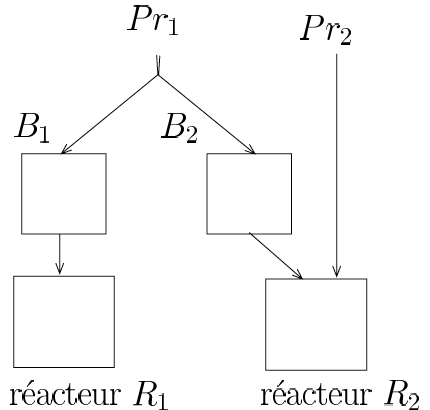
\includegraphics[width=.2\linewidth]{reacteur}
\hspace{.1\linewidth}
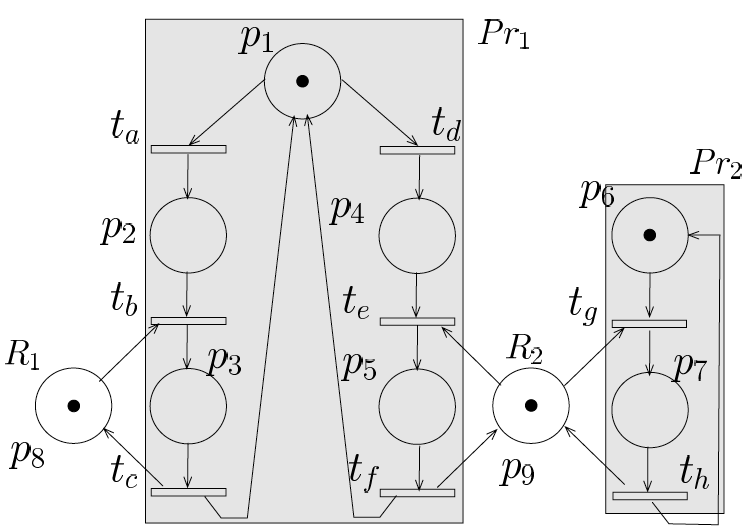
\includegraphics[width=.4\linewidth]{freator}
\end{center}
\end{frame}
 
\subsection{Modèle dynamique}
\begin{frame}{Règle de fonctionnement}
\begin{block}{Transition sensibilisée à partir de M}
	\begin{itemize}
	\item il y a un numéro suffisant de jetons dans les places d'entrée,
	\item $\forall p \in P, \;\;  M(p) \geq Pre(p, t)$
	\item $M \geq Pre(\, . \, ,t)$
	\end{itemize}
\end{block}
\begin{block}{Tir d'une transition à partir de M}
	\begin{itemize}
	\item $\forall p \in P, \;\; M'(p)=M(p)-Pre(p,t)+Post(p,t)$
	\item $M'=M-Pre(\, . \, ,t)+Post(\, . \, ,t)=M + C(\, . \, ,t)$
	\end{itemize}
\end{block}
\end{frame}

\begin{frame}{Règle de fonctionnement}
\begin{columns}
	\begin{column}{.6\linewidth}
		\begin{itemize}
		\item  Enlève $Pre(p,t)$ jetons de chaque place précédente $p$ (poids de l'arc d'entrée), et met $Post(p,t)$ jetons à chaque place de sortie $p$,
		\item  Représente le changement d'état dû à l'ocurrence de l'événement associé à $t$.
		\end{itemize}
	\end{column}
	\begin{column}{.4\linewidth}
		\begin{center}
		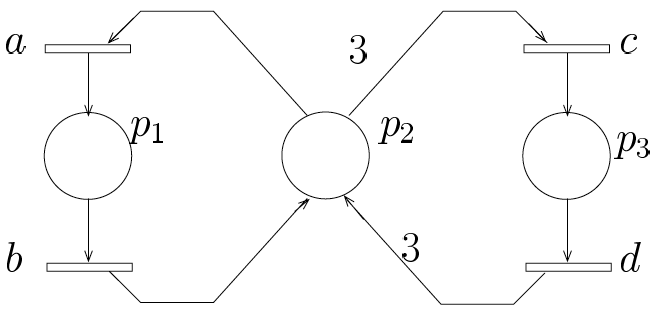
\includegraphics[width=\linewidth]{le}
		\end{center}
	\end{column}
\end{columns}
\end{frame}

\begin{frame}{Conflit et parallélisme}
\begin{itemize}
\item \structure{Conflit structurel :} ssi  $t_1$ et $t_2$ ont au moins une place d'entrée en commun
	$$\exists p \in P, \quad Pre(p,t_1) \, Pre(p,t_2) \neq 0$$
\item \structure{Conflit effectif :} ssi $t_1$ et $t_2$ sont en conflit structurel et sont sensibilisées par le marquage $M$
	$$M \geq Pre(.,t_1) \; \mbox{et} \; M \geq  Pre(.,t_2)$$
\item \structure{Parallélisme structurel :} si $t_1$ et $t_2$ ne possèdent pas de place d'entrée en commun
	$$\forall p \in P \quad Pre(p,t_1) \, Pre(p,t_2) = 0  \;
	\mbox{ou} \; Pre(.,t_1)^T \times Pre(.,t_2) = 0$$
\item \structure{Parallélisme effectif :} $t_1$ et $t_2$ sont parallèles structurellement et
$$M \geq Pre(.,t_1) \; \mbox{e} \; M \geq Pre(.,t_2)$$
\end{itemize}
%$$Pre(.,b) = \begin{pmatrix} 1 \\ 0 \\ 0 \end{pmatrix}$$
%$$Pre(.,d) = \begin{pmatrix} 0 \\ 0 \\ 1 \end{pmatrix}$$
\end{frame}

% \begin{frame}
% \frametitle{Séquence de tir}
%\begin{itemize}
%\item
%$
%\begin{array}{ccccccc}
%  \left[
%  \begin{array}{c}
%  0\\
%  3\\
%  0
%  \end{array}
%  \right] &
%  \stackrel{a}{\longrightarrow} &
%  \left[
%  \begin{array}{c}
%  1\\
%  2\\
%  0
%  \end{array}
%  \right] &
%  \stackrel{a}{\longrightarrow} &
%  \left[
%  \begin{array}{c}
%  2\\
%  1\\
%  0
%  \end{array}
%  \right] &
%  \stackrel{b}{\longrightarrow} &
%  \left[
%  \begin{array}{c}
%  1\\  
%  2\\
%  0
%  \end{array}
%  \right]. \\ M_0 & & M_1 & & M_2 & & M_1
%\end{array}
%$
%\item  $M'$ accessible à  partir de $M$: 
%$M \stackrel{t}{\longrightarrow} M'$,   
%\item $M_0 \stackrel{a}{\longrightarrow} M_1$, 
% $M_1 \stackrel{a}{\longrightarrow} M_2$,
% $M_2 \stackrel{b}{\longrightarrow} M_1$, 
%\item si $M \stackrel{t_1}{\longrightarrow} M'$,   et
%$M' \stackrel{t_2}{\longrightarrow} M''$, on a $s=t_1t_2$ et
%$M \stackrel{t_1t_2}{\longrightarrow} M''$;
%\item
%dans l'exemple, $M_0 \stackrel{s}{\longrightarrow} M_1$, avec $s=aab$, $s$ 
%est dite séquence de tir,
%\item ${\bf s} : T \rightarrow \nat$; ${\bf s}(t)$: nombre 
%d'occurrences de $t$ dans $s$
%\item \fbox{$M'=M+C{\bf s}$} ~ ~ ~ {\color{blue} Équation fondamentale}
%\end{itemize}

% \pause
%Questions:
%\begin{itemize}
%\item étant donné  $M$  et une sequence $s$, il existe $M' ~\mid
%M \stackrel{s}{\longrightarrow} M'$?
%\item étant donné $M$ et $M'$ il existe $s$ tel que $M \stackrel{s}{\longrightarrow} M'$?
%\end{itemize}

% \end{frame}
 

%  \begin{frame}
% \frametitle{Autres représentations}
% {\color{blue} Système de règles}
 
% \vspace{.1cm}
%\begin{itemize}
%\item
%une base de faits, représentant la connaissance disponible sur le système,
%\item
%une base de règles, qui permet de déduire de nouveaux faits,
%\item
%{\em un moteur d'inférence}, qui permet de
%réaliser de nouvelles déductions, appliquant les règles aux faits.
%\end{itemize}

%\vspace{.2cm}
%\noindent
%{\color{blue} Grammaire}

%\vspace{.1cm}
%\begin{itemize}
%\item
%un alphabet $\p$ dont les symboles sont les places $p \in P$, et
%\item
%un ensemble $Q$ de règles de réécriture :\\
%$t: \mu(Pre(.,t)) \rightarrow \mu(Post(.,t)).$
%\item $\mu:  \m \rightarrow {\p}^*$, $\m$ est l'ensemble de tous les marquages et ${\p}^*$ l'ensemble de séquences finies dont la séquence vide $\lambda$
%\item transition sensibilisée : $\mu(Pre(.,t)) \subseteq \mu(M)$,
%\item tir de transition : $\mu(M')=\mu(M) \cup \mu(Post(.,t)) \setminus \mu(Pre(.,t)).$  
%\end{itemize}

% \end{frame}
 
%  \begin{frame}
% \frametitle{Propriétés du modèle : réseau $<\!R,M_0\!>$ borné}
% \begin{itemize}
%\item place k-bornée: $\forall M' \in {\cal A(R},M_0), \;\;\; M'(p) \leq k$\\
%le nombre maximal de jetons pour tout marquage est plus petit que $k$,
%\item si k=1, place binaire,
%\pause
%\item réseau marqué k-borné : ssi toutes les places sont k-bornés,
%\item  réseau marqué binaire : ssi toutes les places sont binaires.
%\end{itemize}
%\begin{center}
%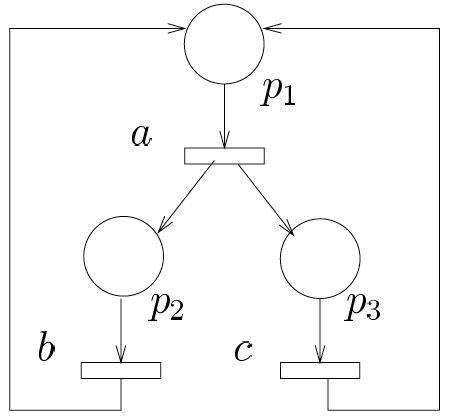
\includegraphics[width=4.5cm]{./figSH/nonbor}
%\end{center}
% \end{frame}
 
 
% \begin{frame}
% \frametitle{Propriétés du modèle : réseau $<\!R,M_0\!>$ vivant}
% \begin{itemize}
%\item Transition {\color{blue}quasi-vivante} : si $ \exists M \in  {\cal A(R},M_0)  \mid
%M \stackrel{t}{\longrightarrow}$\\
%ou : 
%$\exists s \mid M_0 \stackrel{s}{\longrightarrow} M \;\;\; {\rm et}\;\;\; 
%M \stackrel{t}{\longrightarrow}$\\
%($t$ peut être sensibilisée à
%partir de $M_0$ par le tir de la séquence $s$).
%\pause
%\item Transition {\color{blue}vivante} :
%$t$ doit pouvoir être sensibilisée à partir de n'importe quel
%marquage $M$, utilisant une séquence $s$:
%$\forall M \in {\cal A(R},M_0), \; \exists s  \mid \; M \stackrel{st}{\longrightarrow}.$ 
%\pause
%\item Réseau marqué vivant : $N$ est vivant ssi toutes les transitions sont vivantes :
%$\forall t \in T, \; \forall M \in {\cal A(R},M_0), \; 
%\exists s  \mid \; M \stackrel{st}{\longrightarrow}.$
%\end{itemize}

%\begin{center}
%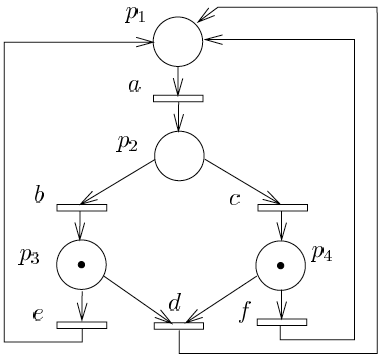
\includegraphics[width=3.9cm]{./figSH/qviva-n}
%\end{center}
%  \end{frame}
  
%   \begin{frame}
% \frametitle{Propriétés du modèle : réseau $<\!R,M_0\!>$ réinitialisable}
% \begin{itemize}
%\item Réseau marqué  {\color{blue}réinitialisable} : il est possible de revenir au
%marquage initial à  partir de n'importe quel marquage: \\
%\[\forall M \in A(R,M_0), \;\;\; \exists s \mid \;\;\;
%M \stackrel{s}{\longrightarrow} M_0.\]
%\end{itemize}
%\begin{center}
%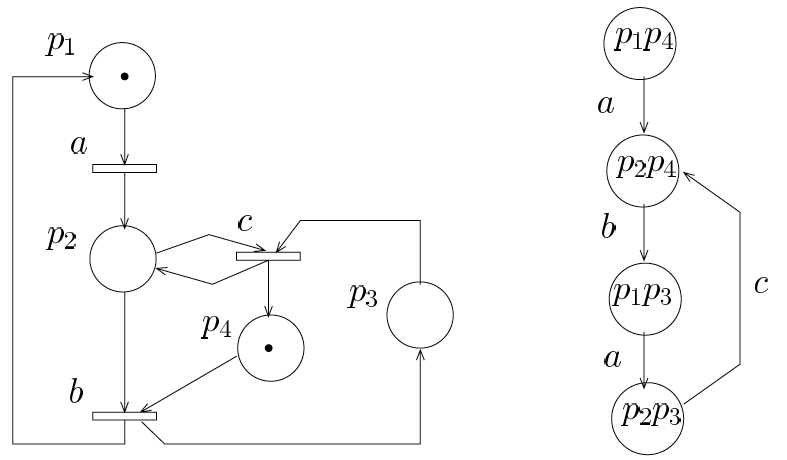
\includegraphics[width=6.5cm]{./figSH/nonrei-g}
%\end{center}
  
%   \end{frame}
  
%   \begin{frame}
% \frametitle{Propriétés structurelles : réseau $R$}
% \begin{itemize}
%\item dérivent directement de la {\em structure} du réseau de Petri,
%\item ne dépendent pas du marquage initial,
%\item composantes + marquage = invariants.  
%\end{itemize}

%\vspace{1cm}
%\noindent
% Composantes {\color{blue}conservatives} et invariants de {\color{blue}place}

%\vspace{1cm}
%\noindent
%Composantes {\color{blue}répétitives} et invariants de {\color{blue}transition}
%  \end{frame}
  
%   \begin{frame}
% \frametitle{Composantes conservatives}
 
% \begin{columns}
%\column{.56\textwidth}
% \begin{itemize}
%\item
%circuit formé par $p_1$, $p_2$, $a$, $b$:\\
%$M(p_1)+M(p_2)$  ne change pas :
%\begin{itemize}
%\item  $M_0= [1\; 0\; 3\; 0\; 1]^T$
%\item $M_0 \stackrel{a}{\longrightarrow}M'= [0\; 1\; 2\; 0\; 1]^T$
%\item $M' \stackrel{b}{\longrightarrow}M''=M_0$
%\end{itemize}
% \end{itemize}
%\column{.44\textwidth}
%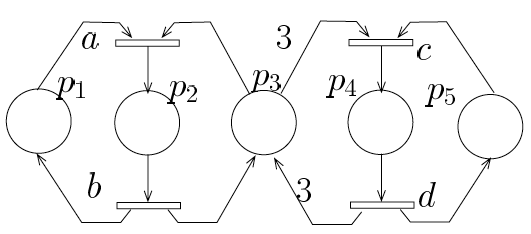
\includegraphics[width=5.2cm]{./figSH/inv}
%\end{columns}
% \begin{itemize}

%\item
%circuit formé par $p_2$,$p_3$ et $p_4$, $a$,$b$,$c$ et $d$ :\\
%$M(p_2)+M(p_3)+3.M(p_4)=$ cte:\\
%\item
%fonctionnement dynamique  de $R$ est donné par $M'=M+C{\bf s}$ : \\
%pour obtenir une somme pondérée de
%marquages \\
%$\leadsto$ multiplier l'éq. par ${\bf f}^T$:
%$~~~{\bf f}^TM' = {\bf f}^TM + {\bf f}^TC\bf{s}$
%\item pour que lŽéquation soit indépendante des séquences de tir $s$: \\
%annuler le produit ${\bf f}^TC$.
%\item composante conservative : ${\bf f}^TC = 0$ $\leadsto$ défini un sous-réseau de Petri  
% \pause
%\item dans l'exemple : \\
%${\bf f}^1=[\,1~1~0~0~0\,]^T$, ${\bf f}^2=[\,0~1~1~3~0\,]^T$ et
%${\bf f}^3=[\,0~0~0~1~1\,]^T.$
%\end{itemize}

%  \end{frame}
  
%   \begin{frame}
% \frametitle{Invariants de place}
% \begin{itemize}
%\item Invariants de place
% = composante conservative + marquage\\
%  (la composante conservative est une information {\color{blue} structurelle})
%\item
%comme  ${\bf f}^TC = 0$,  on a ${\bf f}^TM = {\bf f}^TM_0 \;\;\forall M \in
%A(R,M_0)$\\
%$\leadsto$ invariant de place
% \pause
%\item $M(p_1) + M(p_2) = M_o(p_1) + M_o(p_2)=1$
%\item $M(p_2) + M(p_3) + 3.M(p_4) = 3$  
%\item $M(p_4) + M(p_5) =1$  
%\end{itemize}

%\vspace{.1cm}
%\noindent
%{\bf Remarque} 

%\begin{itemize}
%\item
%composante conservative : dépend seulement de la structure !
%\item
%invariant de place : dépend de la  {\color{blue}structure} {\bf et} du  {\color{blue}marquage}.  
%\end{itemize}

%  \end{frame}
  
%   \begin{frame}
% \frametitle{Composantes répétitives stationnaires}
 

% \begin{itemize}
%\item sous-réseau formé par $c$ et $d$, et places $p_3$, $p_4$ et $p_5$:\\
%tir de $s=cd$ à partir de $M_0$ ramène au même marquage !
%\item
%transitions $c$ et $d$ forment une composante répétitive stationnaire.
%\item
%fonctionnement dynamique  $M'=M+C{\bf s}$: pour que $M'=M$, $C{\bf s}=0$
%\item solution $\bf{s}$:  {\em composante répétitive}
% $\leadsto$ définit un sous-réseau
%avec transitions ${\bf s}(t) \neq 0$, et places d'entrée et sortie,
%\item dans l'exemple: ${\bf s}^1=[\,1~1~0~0\,]^T$, ${\bf s}^2=[\,0~0~1~1\,]^T$ 
%\end{itemize}

%\begin{center}
%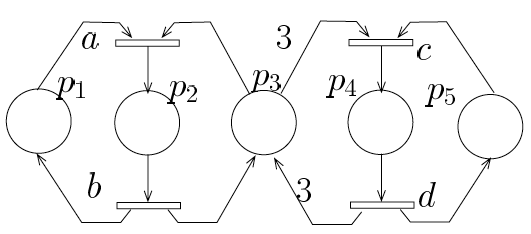
\includegraphics[width=5.2cm]{./figSH/inv}
%\end{center}
%  \end{frame}
  
%     \begin{frame}
% \frametitle{Invariants de transition}
 
%\begin{itemize}
%\item séquences $s_i$ obtenues à partir du vecteur ${\bf s}$
%\item pour ${\bf s_1}$ on a les invariants $s_1=ab$, $s_2=ba$: tous les
%  invariants ne correspondent pas forcement à une séquence possible !!
%\item il faut calculer $M \stackrel{ab}{\longrightarrow}$ et
%$M \stackrel{ba}{\longrightarrow}$ pour vérifier !
%\end{itemize}  

%\vspace{.1cm}
%\noindent
%{\bf Remarque} 

%\begin{itemize}
%\item
% composante répétitive : dépend seulement de la structure !
%\item
%invariant de transition : dépend de la  {\color{blue}structure} {\bf et} du  {\color{blue}marquage} (besoin de calculer $M \stackrel{s_i}{\longrightarrow}$).  
%\end{itemize}
%  \end{frame}
  
 
%  \begin{frame}
% \frametitle{Exemple : Système par lot}
% {\color{blue} Composantes conservatives:}

%\vspace{.2cm}
% ${\bf f}^1=[\,1~1~1~1~1~0~0~0~0\,]^T$,
%${\bf f}^2=[\,0~0~0~0~0~1~1~0~0\,]^T$, ${\bf f}^3=[\,0~0~1~0~0~0~0~1~0\,]^T$,
%${\bf f}^4=[\,0~0~0~0~1~0~1~0~1\,]^T$, \\
%qui définissent les réseaux :

%\vspace{.2cm}
%\begin{itemize}
%\item
% $p_1$, $p_2$, $p_3$, $p_4$ et $p_5$, et  $t_a$, $t_b$,
%$t_c$, $t_d$, $t_e$ et $t_f$:  2 options  de fab. de $Pr_1$;
%\item
%$p_6$ et $p_7$,  $t_g$ et $t_h$: fabrication du produit $Pr_2$;
%\item
%$p_3$ et $p_8$,  $t_b$ et $t_c$:  les évolutions de l'état du réacteur $R_1$;
%\item
% $p_5$, $p_7$ et $p_9$, $t_e$, $t_f$, $t_g$ e $t_h$:
%les évolutions de l'état du réacteur $R_2$.
%\end{itemize}

%\begin{center}
%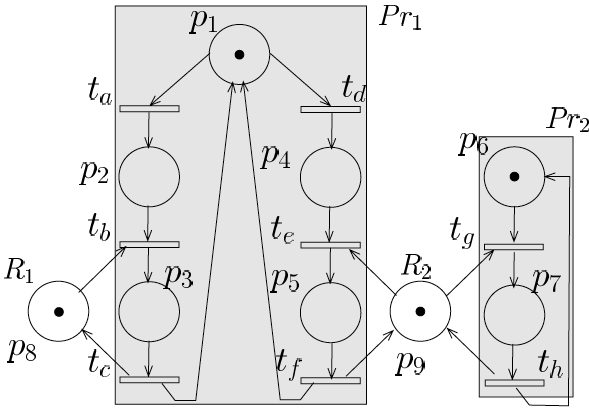
\includegraphics[width=5.2cm]{./figSH/rea1}
%\end{center}

% \end{frame}

% \begin{frame}
% \frametitle{Exemple : Système par lot}
% {\color{blue} Invariants de place (pour $M_0 = p_1p_8p_9$) :}


%\vspace{.1cm}
%\begin{itemize}
%\item
%$I_1$:   $M(p_1)+M(p_2)+M(p_3)+M(p_4)+M(p_5)=1$: lot  $Pr_1$  en attente
% ($p_1$),  en $B_1$ ($p_2$), en $B_2$ ($p_4$), dans $R_1$  ($p_3$) ou $R_2$ ($p_5$),
%\item
%$I_2$: $M(p_6)+M(p_7)=1$: \\
%existe un lot $Pr_2$ en attente ($p_6$) ou dans
%$R_2$ ($p_7$);
%\item
%$I_3$: $M(p_3)+M(p_8)=1$: \\
%$R_1$ libre ($p_8$) ou en cours de proc. dans $Pr_1$ ($p_3$);
%\item
%$I_4$: $M(p_5)+M(p_7)+M(p_9)=1$:  \\
%$R_2$ libre ($p_9$), en cours proc. dans
% $Pr_1$ ($p_5$) ou  $Pr_2$ ($p_7$).
%\end{itemize} 
  
% \begin{center}
%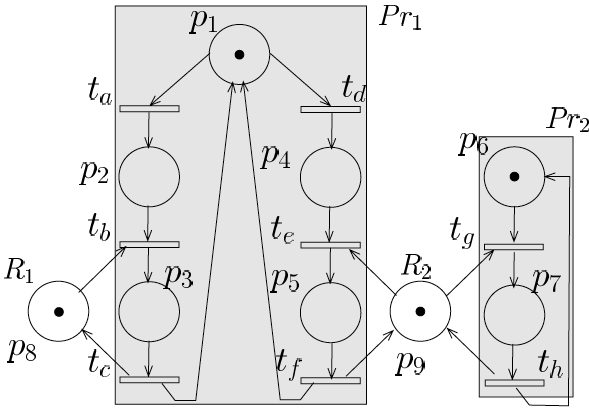
\includegraphics[width=4.8cm]{./figSH/rea1}
%\end{center}
% \end{frame}
 
% \begin{frame}
% \frametitle{Exemple : Système par lot}
% {\color{blue} Composantes répétitives stationnaires} 

%\vspace{.1cm}
% \begin{itemize}
%\item
%vecteurs ${\bf s}^1=[\,1~1~1~0~0~0~0~0\,]^T$,
%${\bf s}^2=[\,0~0~0~1~1~1~0~0\,]^T$ et
%${\bf s}^3=[\,0~0~0~0~0~0~1~1\,]^T$,
%\item
%$t_a$, $t_b$ e $t_c$, avec  $p_1$, $p_2$, $p_3$ et $p_8$: 
% le lot $Pr_1$ passe par le {\em buffer} et est proc. par $R_1$; un
%nouveau cycle peut recommencer ;
%\item
%$t_d$, $t_e$ et $t_f$ +  $p_1$, $p_4$, $p_5$ et $p_9$: même comportement
%\% à $Pr_2$ et $R_2$;
%\item
%$t_g$ et $t_h$, avec  $p_6$, $p_7$ et $p_9$: séquence
%d'événements début de proc. de $Pr_2$ \mbox{et fin.}
%\end{itemize} 

%\begin{columns}
%\column{.6\textwidth}

%\vspace{.07cm} {\color{blue} Invariants de transition \\
%(pour $M_0 = p_1p_8p_9$) :}
%\vspace{.1cm}
%\begin{itemize}
%\item $s_1=t_at_bt_c$, $s_2=t_dt_et_f$ et $s_3=t_gt_h$ :\\
% les seules séquences effectivement tirables !
%\end{itemize} 
 
%\column{.4\textwidth}
%\begin{center}
%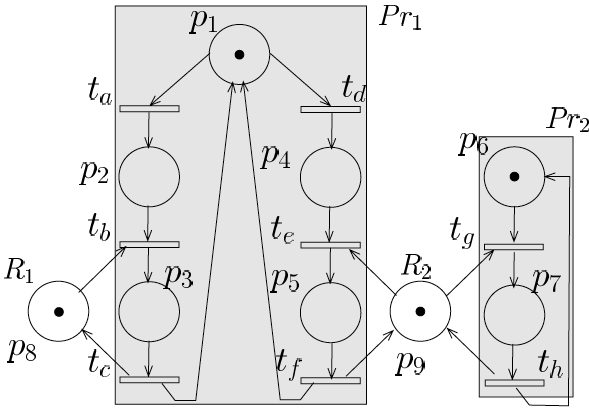
\includegraphics[width=4.8cm]{./figSH/rea1}
%\end{columns}

% \end{frame}

% \subsubsection{Analyse des propriétés}
 
%   \begin{frame}
% \frametitle{Analyse des propriétés}
%\begin{description}
%\item[Analyse par énumération de marquages]
%le graphe de marquages accessibles est calculé, vérifiant si le réseau est borné, vivant et reinitialisable.
% \pause
%\item[Analyse structurelle]
%calcul des composantes conservatives et répétitives stationnaires et des
%invariants correspondants.
%Ne permet pas toujours d'avoir une réponse, mais dans certains cas, permet d'obtenir une réponse simples et rapide des propriétés du réseau.
%   \pause
%\item[Analyse par réduction]
%si le réseau est trop grand ou non borné, on peut réduire la taille du réseau,
%en utilisant certaines règles de réduction.
%\end{description}  
%  \end{frame}
 
%  \begin{frame}
% \frametitle{Analyse par énumération des marquages}
% {\color{blue}Arbre de couverture}
 
% \vspace{.2cm}
%\begin{itemize}
%\item
%on part du marquage initial  $M_0$,
%\item chaque transition sensibilisée par $M_0$  donne origine à une branche,
% \pause
%\item la construction d'une branche est interrompue quand on rencontre un marquage 
%\begin{itemize}
%\item
%déjà calculé et pour lequel tous les successeurs ont été déjà 
%calculés ou seront calculés (branche pendante à être explorée) :
%\item
%strictement supérieur à un marquage
%{\em de la branche qui est en train d'être explorée}
%(le réseau peut être non borné) $\rightarrow M(p)=\omega$.
%\end{itemize}  
%\end{itemize}  
%Si le réseau est non borné, l'arbre est fini dû à l'introduction du symbole $\omega$.
% \end{frame}  
 
%   \begin{frame}
% \frametitle{Analyse par énumération des marquages}
%  {\color{blue} Recherche des propriétés d'un réseau $N=<\!{\cal R},M\!>$ \\
%  sur le graphe ${\cal A(R},M)$}
  
%   \vspace{.2cm}
%\begin{itemize}
%\item réseau $k$-borné : graphe ${\cal A(R},M)$  est borné,
% \pause
%\item réseau réinitialisable :  graphe fortement connexe:
%$ \forall M_i,M_j \in {\cal A(R},M),~ \exists s \mid M_i
%\stackrel{s}{\rightarrow} M_j$ (existe un chemin entre n'importe quelle paire de noeuds),
% \pause
%\item
%réseau vivant :  graphe fortement connexe et toutes les transitions étiquetent au moins un des arcs :
%$ \forall t  \in T ~\exists M_i,~\exists M_j \in {\cal A(R},M),~ \mid M_i
%\stackrel{t}{\rightarrow} M_j.$

%\end{itemize}  

% \end{frame}  
 
%   \begin{frame}
%  \frametitle{Analyse par énumération des marquages}
%  {\color{blue}Pas pour l'analyse}

%\begin{enumerate}
%\item
%vérifier si le réseau marqué est borné (arbre
% de couverture) ;
%\item
%si le réseau marqué est borné, construire le graphe de marquages accessibles ;
%\item
%montrer que ce graphe est fortement connexe ;
%\item
%vérifier que chaque transition apparaît au moins une fois comme étiquette d'un arc du graphe de marquages accessibles.
%\end{enumerate}

%\noindent
%$\leadsto$ vérifier si le réseau {\color{blue} marqué} est en même temps
%borné, reinitialisable et vivant.

%\begin{center}
%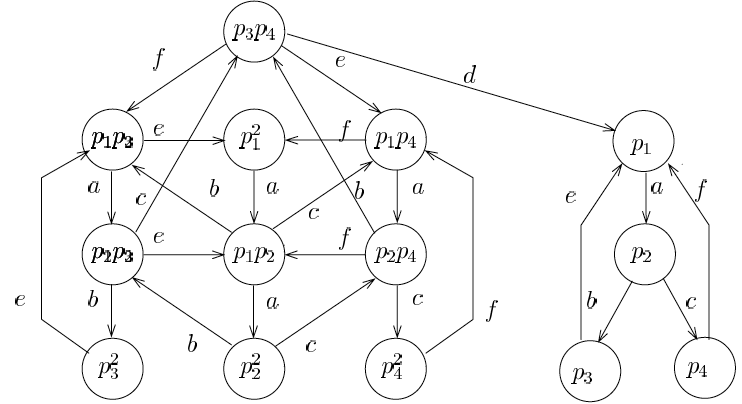
\includegraphics[width=5.6cm]{./figSH/qviva-g}
%\end{center}
% \end{frame}  
 
 

%  \begin{frame}
% \frametitle{Analyse  des propriétés  structurelles}
 
%   {\color{blue}Réseau non marqué : composantes conservatives}

%\begin{itemize}
%\item
%toute place qui  {\color{blue}appartient} à une composante conservative  {\color{blue}est} bornée ;
%\item
%une place $p$ qui {\color{blue} n'appartient} à aucune composante conservative
%($f(p)=0$)  {\color{blue}peut} être bornée ;
%\item
%une place non bornée n'appartient à aucune  composante conservative
%\end{itemize}

% Un réseau de Petri pour
%lequel il existe une couverture de composantes 
%conservatives $f^T>0$ est
%k-borné, {\it peu importe son marquage initial.}

% \pause
%\vspace{.4cm}  
%\noindent
% {\color{blue} Réseau marqué : invariants de place}

%$f^TM = f^TM_0$ permet de calculer une limite pour  {\color{blue}chaque} place $p$:
%
%\vspace{.3cm}  
%\begin{center}
%\fbox{\rule[-.5cm]{0cm}{1cm}
%$f(p) M(p) \leq f^T M_0,~~M(p) \leq \frac{f^TM_0}{f(p)}$}  
%\end{center}
%    \end{frame}  
    
%      \begin{frame}
% \frametitle{Analyse  des propriétés  structurelles}
 
%   {\color{blue}Réseau non marqué : composantes répétitives}

%\vspace{.3cm}  
%Réseau de Petri répétitif : réseau  pour
%lequel il existe une couverture de composantes 
%répétitives $s>0$ 
%\begin{itemize}
% \pause
%\item
%un réseau de Petri borné et vivant   {\color{blue}est} répétitif \\
%(la réciproque n'est pas vraie)
%
% \pause
%\item un réseau répétitif ($\forall t, ~s(t) > 0$) peut être non vivant
%(une transition  qui  {\color{blue}appartient} à une composante répétitive  {\color{blue}n'est pas} forcement vivante)
% \pause
%\item si le réseau est non répétitif ($\exists t, ~s(t) =0$), le réseau est non vivant  {\color{blue}ou} non borné (une transition  qui {\color{blue} n'appartient pas} à une composante répétitive  est non vivante {\color{blue}ou} amène à un marquage non borné)
% \pause
%\item
%une transition non vivante peut donc appartenir à une  composante répétitive...
%\end{itemize}


%\end{frame}  
   
% \begin{frame}
% \frametitle{Exemples}

% \begin{columns}
%\column{.56\textwidth}
 
% Réseau borné et réinitialisable (pour $M_o=p_1$) mais $t_3$ non vivante 
 
%      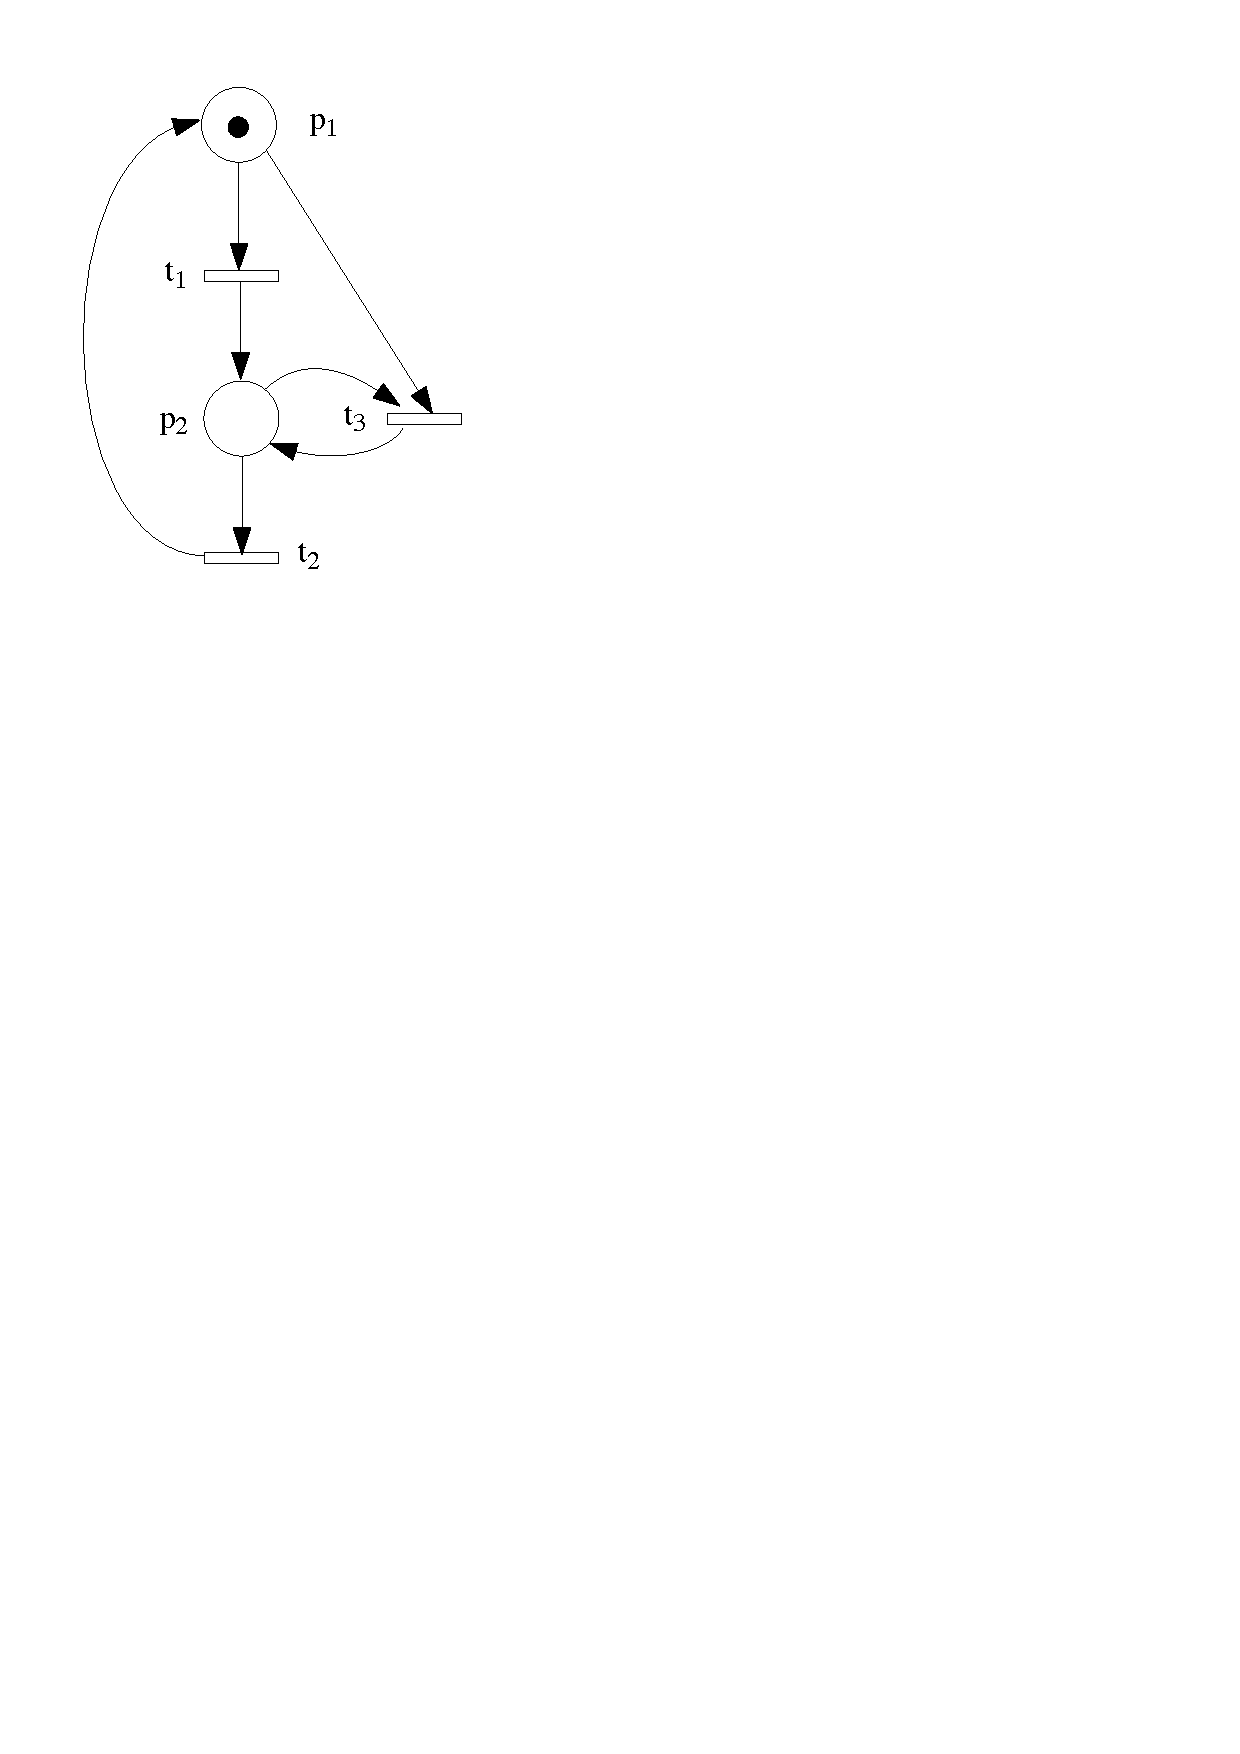
\includegraphics[width=3cm]{./figSH/exemplea} 
      
%      \vspace{.3cm}
      
       
%      \column{.56\textwidth}
%       Réseau non vivant mais toutes les transitions appartienent à une  composante répétitive
%       \\
%  \includegraphics[width=3.4cm]{./figSH/blocage1_ndr}
%     \end{columns} 
%     \end{frame}      
 
 
% \subsubsection{Caractéristiques : modularité, composition, calculabilité}
 
%   \begin{frame}
% \frametitle{Caractéristiques de la représentation par RdP}
% \begin{itemize}
%\item  {\color{blue}Modularité} : est-il possible de décomposer un système complexe?
%\item  {\color{blue}Composition} : si les modules ont les bonnes propriétés, la composition de ces modules garde-t-elle les bonnes propriétés? Ou est-il nécessaire d'analyser le système globale (composé)?
%\item  {\color{blue}Calculabilité} : existe-t-il des algorithmes pour l'analyse? %Et pour l'exécution? (???)
%\end{itemize}

% \vspace{.2cm}
% {\color{blue} Bloc bien-formé}  ({\it module})   \\ 
% un réseau de Petri avec :
% \begin{itemize}
%\item une transition d'entrée $t_e$ et une transition de sortie $t_s$,
%\item réseau borné, vivant et réinitialisable si l'on rajoute une place $p$ tel que $Pre(p,t_e)=Post(p,t_s)=1$. \\
%Ex: séquence, if-then-else, do-while, fork-join.
%\end{itemize}

%   \end{frame}
 
%  \begin{frame}
% \frametitle{Raffinement}
 
%Processus d'abstraction fait en deux temps :

% \vspace{.2cm}
% \begin{itemize}
%\item modélisation d'une  première ébauche ({\it vision abstraite du système global}), avec des transitions {\it abrégées} (associées à des tâches complexes),
%\item à partir de ce RdP, remplacer les  transitions {\it abrégées} par  des  {\color{blue} blocs bien-formés} représentant une vision détaillée de ces tâches complexes
%\item conception {\it top-down}
%\item analyse : si le réseau abstrait est un bloc bien formé, et les transitions sont représentées par des blocs bien formés, alors le réseau global est bien formé.
%\end{itemize} 
% \end{frame}
%
 
%  \begin{frame}
% \frametitle{Composition}
  
%  Processus "à objets" :
%  \begin{itemize}
%\item modélisation  {\color{blue} détaillée} de deux objets dès le départ
%\item construction du réseau global à partir de la composition de ces objets
%  \begin{itemize}
%  \item Composition {\color{blue} asynchrone} (fusion des places)
% \item Composition {\color{blue} synchrone} (fusion des transitions)
% \end{itemize}

%\item conception {\it botton-up}
%\item analyse : le réseau global composé ne conserve pas forcement les propriétés de chaque bloc
%\end{itemize}


%  \end{frame}
  
% \begin{frame}
% \frametitle{Composition}
%  \begin{small}
  
%   \begin{columns}
%\column{.3\textwidth}
% {\color{blue} \bf Composition synchrone} 
 
%  Fusion des transitions $t_1$ et $t_3$ ($t_{13}$) et de\\
%  $t_2$ et $t_4$ ($t_{24}$).
  
%   \vspace{.2cm}
%  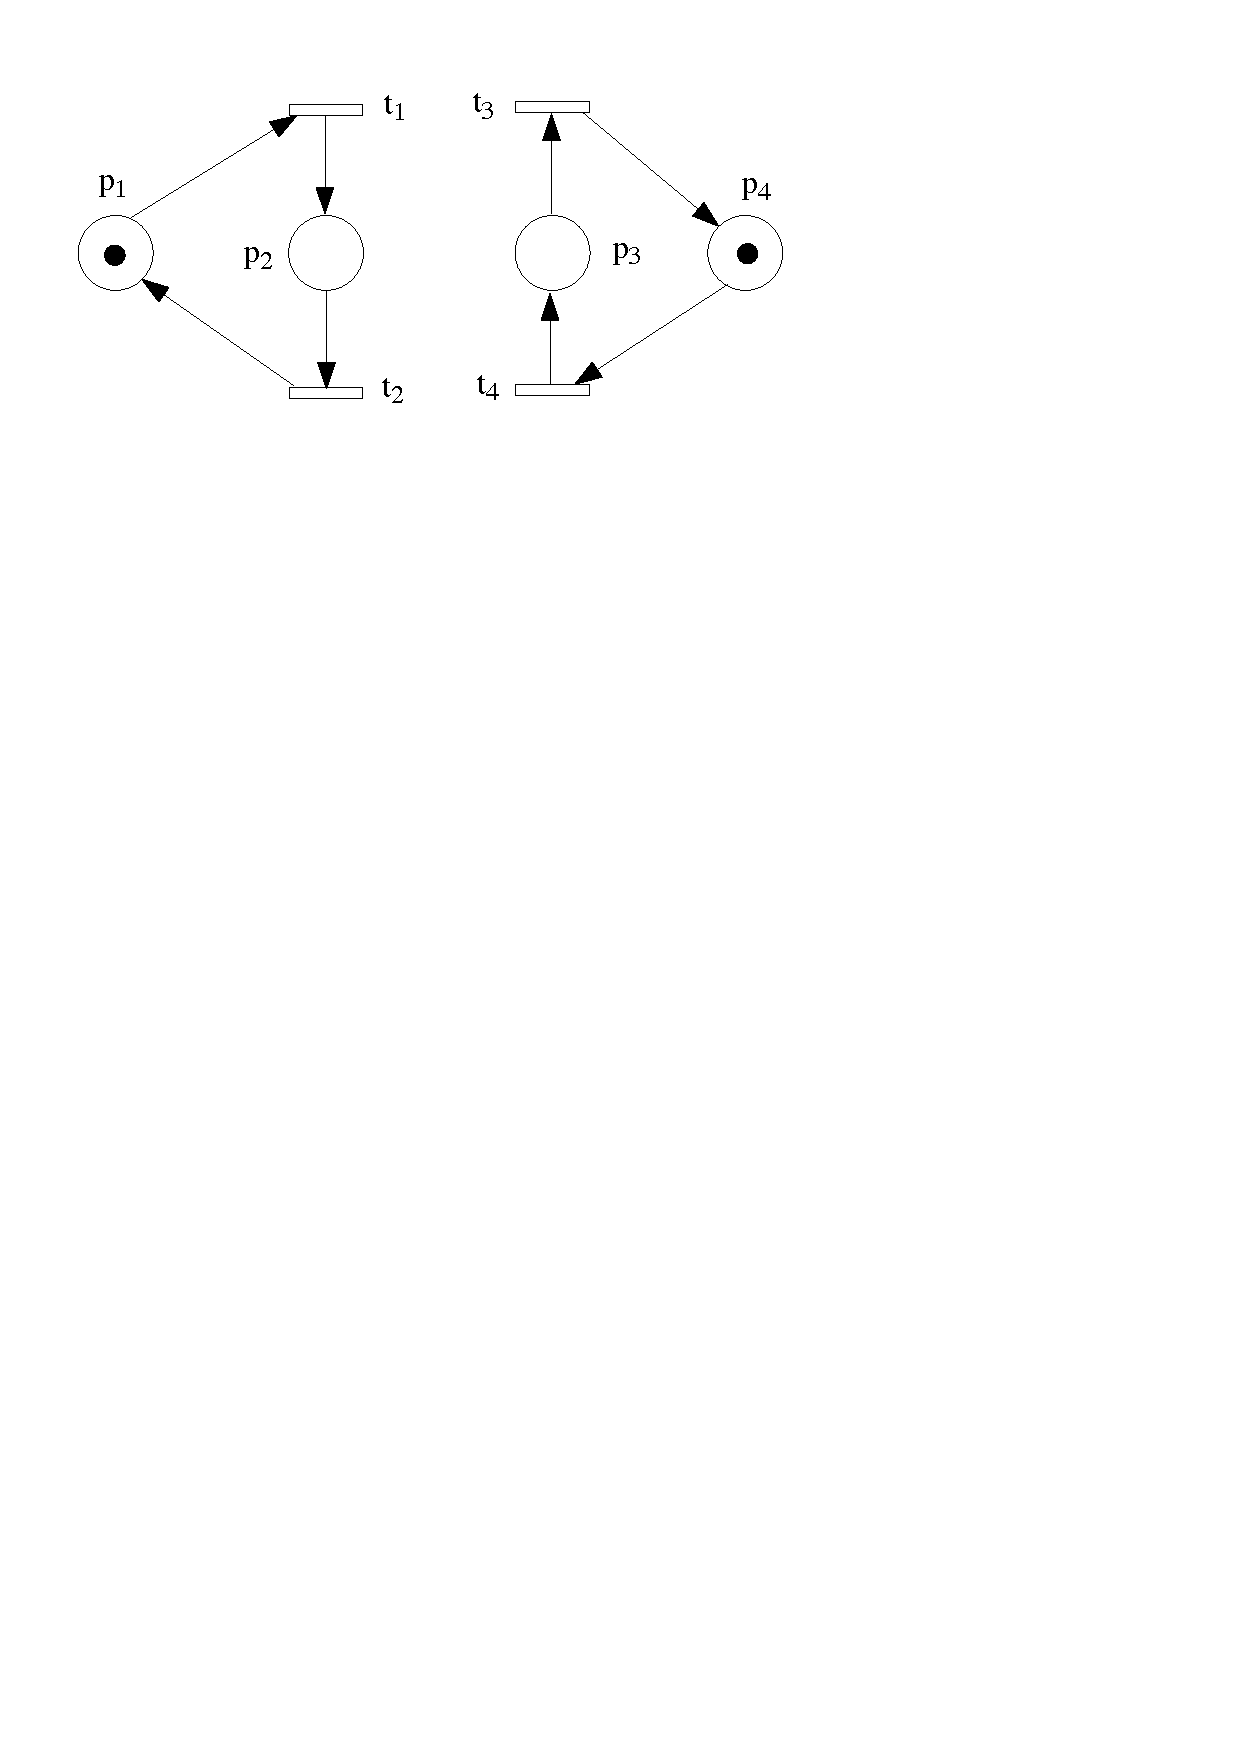
\includegraphics[width=4cm]{./figSH/compoa} 
  
%  \pause
%   \column{.7\textwidth}
%      {\color{blue} \bf Composition asynchrone} : \\
%      Fusion des places $p_2$ et $p_7$ ($p_{27}$).
  
  
% 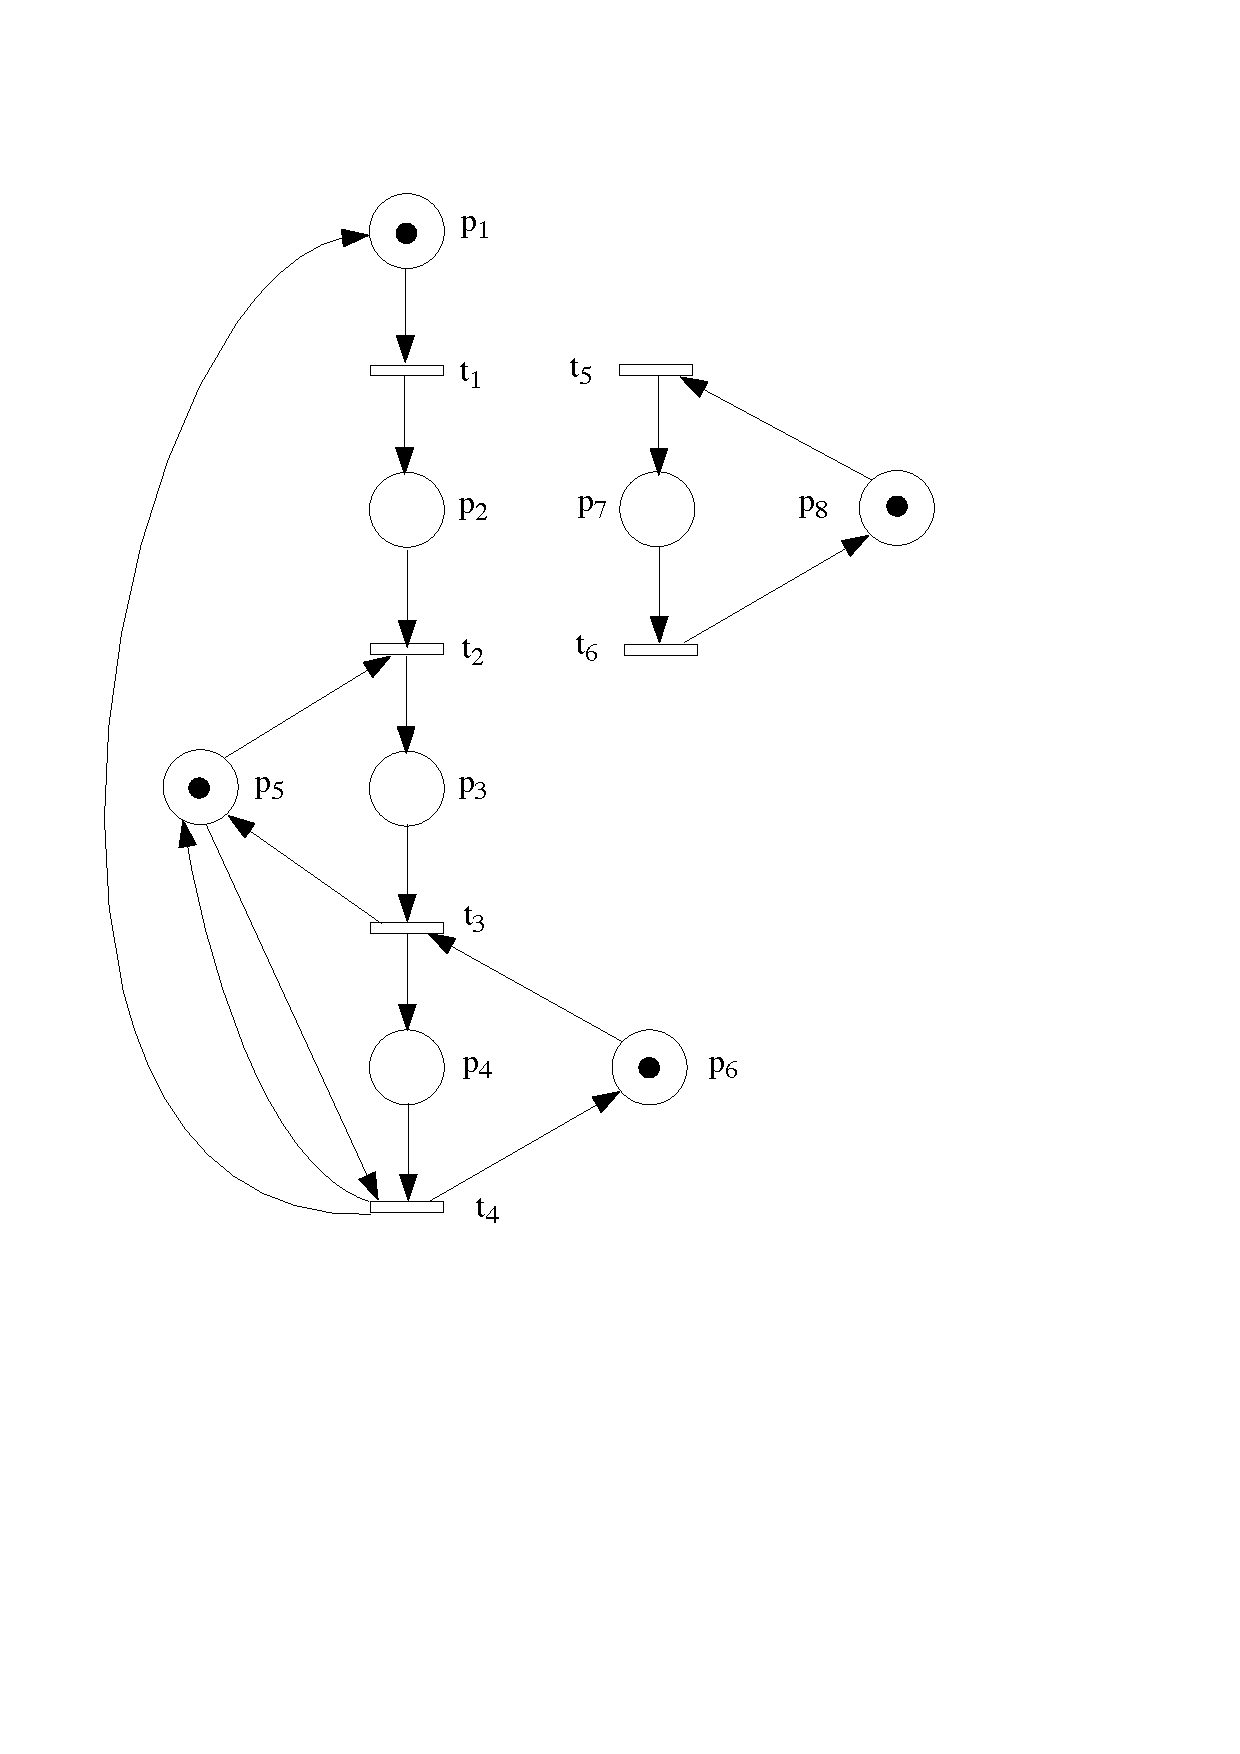
\includegraphics[width=5cm]{./figSH/exempleb}  
%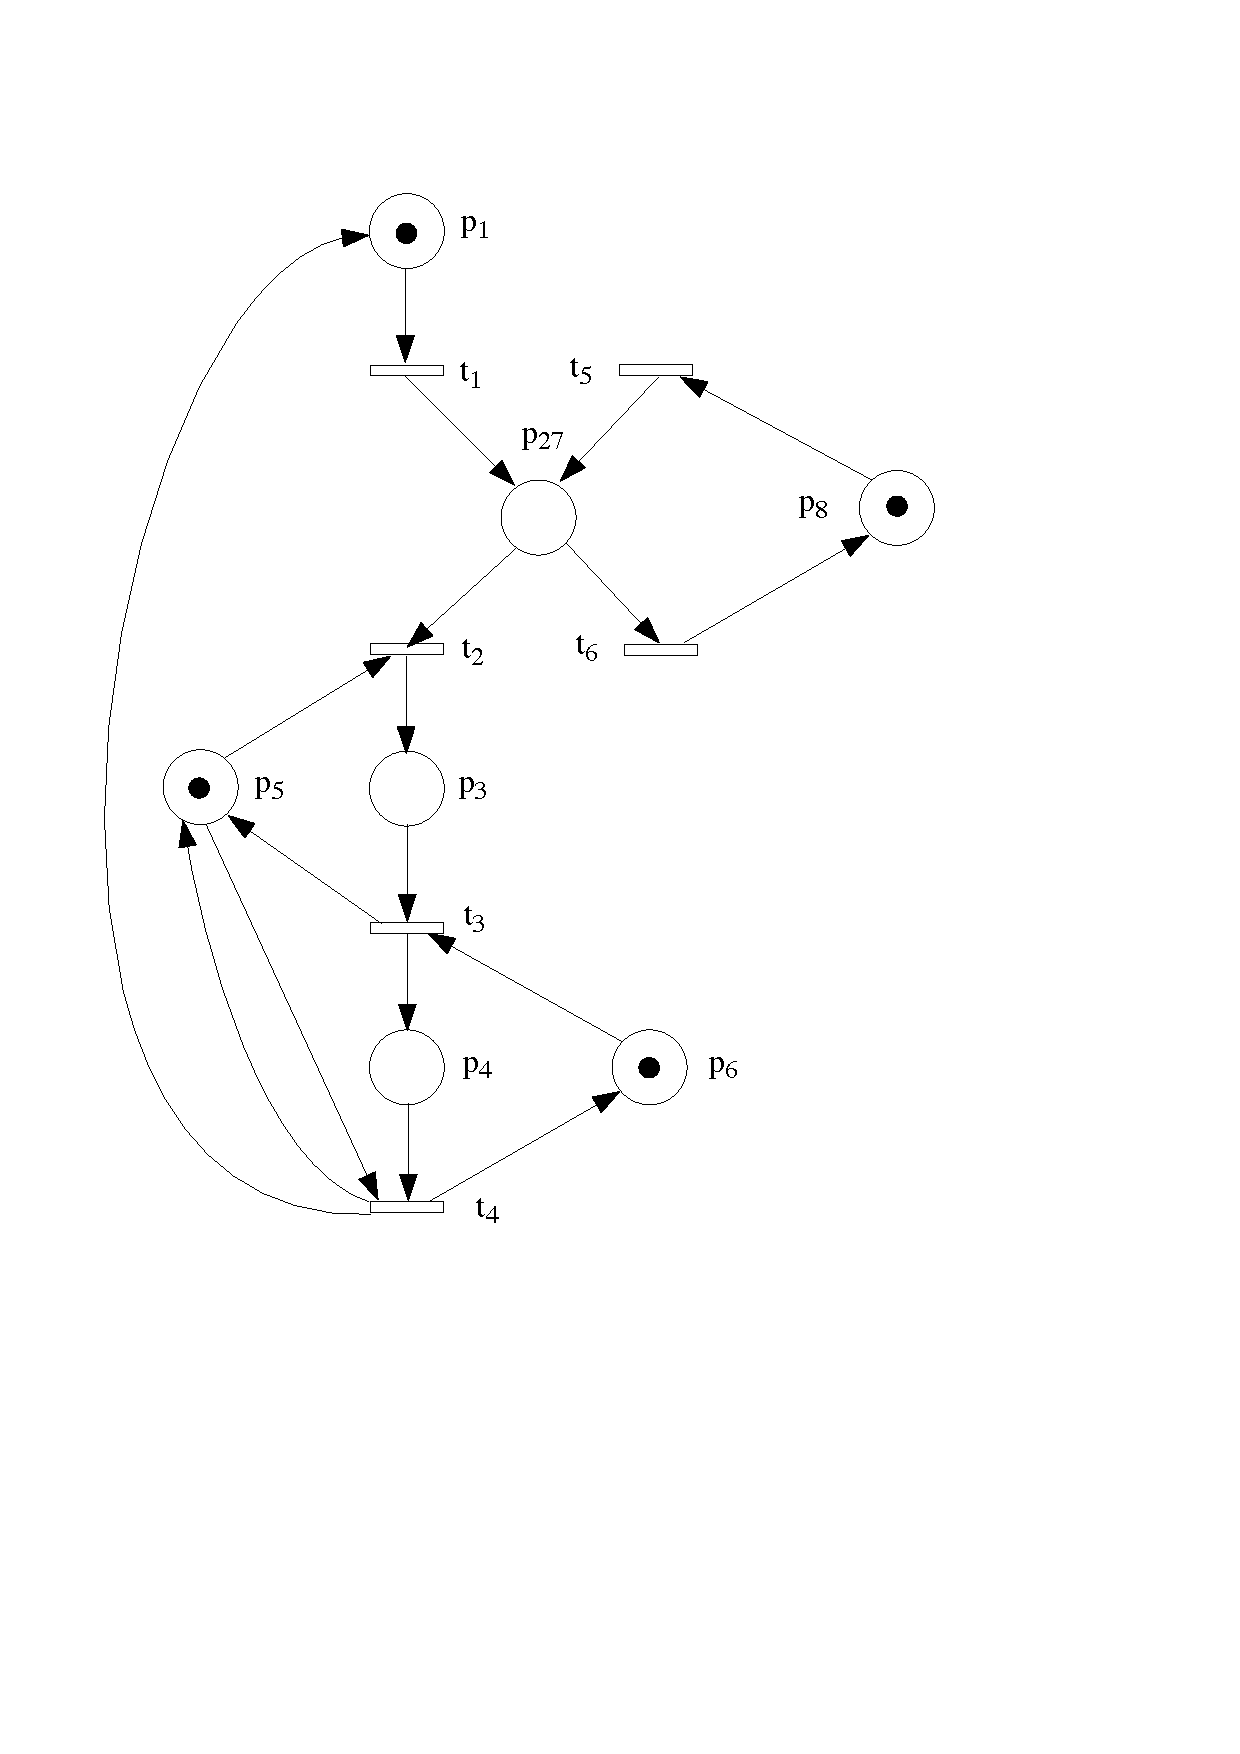
\includegraphics[width=5cm]{./figSH/exemplec} 
%   \end{columns}
%   \end{small}
% \end{frame}



%  \begin{frame}
% \frametitle{Communication par place}
%Deux processus $A$ et $B$ exécutant chacun une opération doivent se communiquer :\\
%$\bullet$ $A$ ne peut commencer qu'après la fin de $B$ ;\\
%$\bullet$ $B$ doit attendre que $A$ commence pour pourvoir commencer.\\

%  \begin{small}  \begin{columns}
%\column{.27\textwidth}
%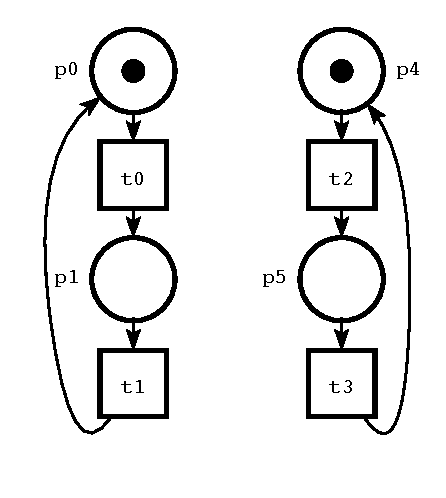
\includegraphics[width=3.2cm]{./figSH/comp2Seul_ndr}\\
%si les processus étaient indépendants \pause
%\column{.35\textwidth}
% 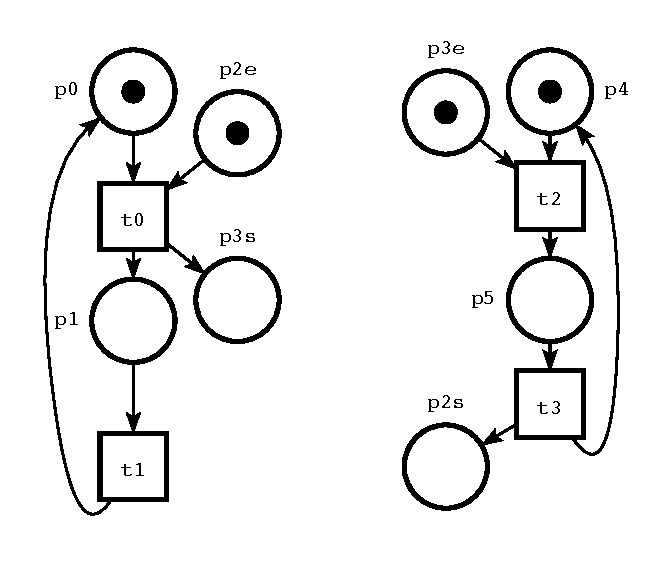
\includegraphics[width=4.4cm]{./figSH/compSep_ndr} \\
% modèle local avec communication\pause
% \column{.3\textwidth}
%    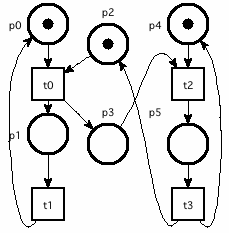
\includegraphics[width=3.5cm]{./figSH/comp3_ndr}\\
%    modèle global avec fusion de places
%   \end{columns}
%     \end{small}
%      \end{frame}

 
%  \begin{frame}
% \frametitle{Tina toolbox}
% 
% \begin{small}
% Tina is a toolbox for the edition and analysis of Petri Nets and Time Petri Nets, developed in the OLC group of LAAS/CNRS.
% \begin{itemize}
%\item ouvrir une fenêtre de commandes en ligne ; taper "nd" (NetDraw)
%\item faire Help, Setup (5eme ascenceur): indiquer le nombre de boutons de la souris
%\item faire Help, Help : comment créer les  places, les transitions, les arcs, comment changer les propriétés d'une place (marquage, label), d'un arc (poids), d'une transition (label). Comment déplacer, effacer les éléments...
%\item éditer le RdP des lecteurs écrivains
%\item générer le graphe d'accessibilité (tools/reachability analysis/ cocher "marking graph", utiliser comme sortie "lts(.aut)".
%\item dessiner ce graphe : click droit, "open file in nd" ; edit/draw ; déplacer les noeuds pour que le graphe soit lisible, et "séparer" les doubles flèches
%\item générer le graphe d'accessibilité (tools/reachability analysis/ cocher "marking graph", utiliser comme sortie "verbose".
%\end{itemize}
% \end{small}
% \end{frame}
%  \begin{frame}
% \frametitle{Retour aux RdP : composition synchrone}
% {\footnotesize À partir des RdP représentant les philosophes (P et Q) et les baguettes (1 et 2), construire le RdP du système global (partage des baguettes par les 2 philosophes) en utilisant la composition synchrone (fusion des transitions avec le même nom ou correspondant au même événement)}
 
% \begin{columns}
%\column{.5\textwidth}  
%\pause
%{\scriptsize \hspace{1cm}P \hspace{3cm}Q~~~}\\
%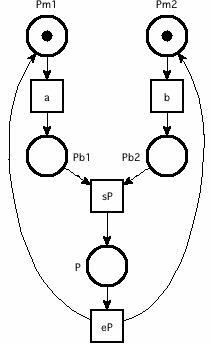
\includegraphics[width=3cm]{figSH/philP_ndr}
%    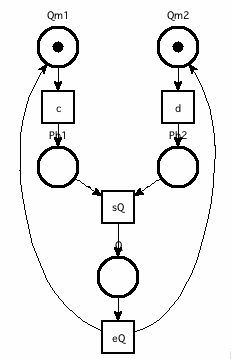
\includegraphics[width=3.2cm]{figSH/philQ_ndr}  % PQ
%    \column{.5\textwidth}
%    \pause
%    {\scriptsize \hspace{1cm}b1 \hspace{2.2cm}b2~~~}\\
%      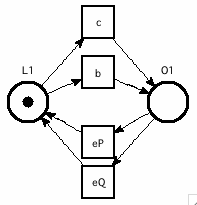
\includegraphics[width=2.5cm]{figSH/baguette1_ndr} 
%           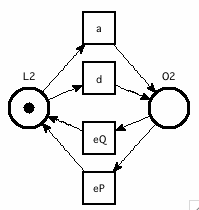
\includegraphics[width=2.5cm]{figSH/baguette2_ndr} \\
% {\scriptsize           Fusion de $t$ de $R_1$ avec  $t$ de $R_2$ : $t_{12}$\\
% \begin{itemize}
% \item soit $p \in R_1$ et $q \in R_2$ ; $r \in R_{12}$
%\item Pre$(r,t_{12})$=Pre$(p,t_1)$ et Pre$(q,t_2)$
%\item Post$(r,t_{12})$=Post$(p,t_1)$ et Post$(q,t_2)$
%\end{itemize}
%}
%           \end{columns}
% \end{frame}

%  \begin{frame}
% \frametitle{Retour aux RdP : composition synchrone}
% \begin{columns}
%\column{.6\textwidth}
% {\footnotesize RdP global PQb1b2 obtenu par composition synchrone de P, Q, b1 et b2}
%  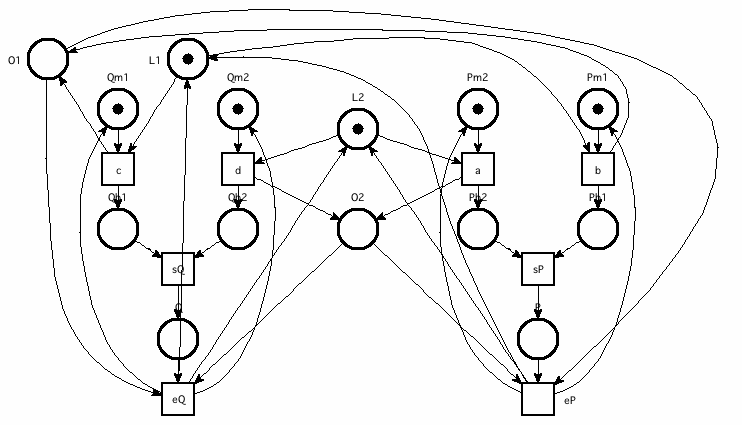
\includegraphics[width=7cm]{figSH/PQb1b2_ndr}
%\column{.4\textwidth}
% {\footnotesize Graphe de marquage du RdP PQb1b2 = automate pg~60}\\%\pageref{phil_aut}
%  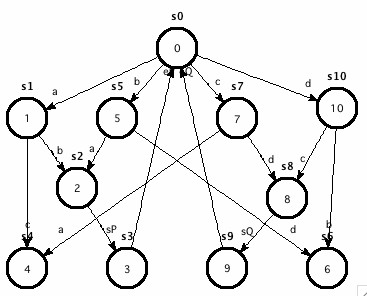
\includegraphics[width=4cm]{figSH/PQb1b2_aut}
%\end{columns}
% \end{frame}
%\subsection{Réseau de Petri et le temps}
% \begin{frame}
% \frametitle{Réseau de Petri et le temps}
 
% Plusieurs extensions de RdP pour prendre en compte le temps :
% \begin{itemize}
%\item temps  associé aux arcs,
%\item temps associé aux places,
%\item temps associé aux transitions (RdP temporel, RdP temporisé)
%\end{itemize}

%\vspace{.5cm}
%Réseaux de Petri temporels (Merlin, 1974)
%\includegraphics[width=4cm]{figCharles/rdp_s_entre}~~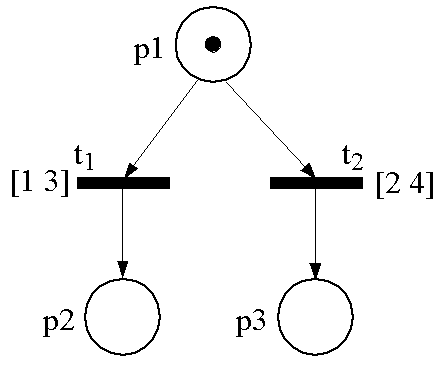
\includegraphics[width=4cm]{figCharles/rdp_s_forte}
% \end{frame}
 
 
% \begin{frame}
%\frametitle{Réseaux de Petri t-temporels ~1/3}

%\only<1>{\vspace{1ex}Un réseau de Petri t-temporel $<N, M_0, I>$
%est défini par~:
%\begin{itemize}
%    \item un réseau de Petri \mbox{$N = <P,T,Pre, Post>$},
%    \item un marquage initial $M_0$,
%    \item  une fonction intervalle statique $I$ :
%    \mbox{$T \rightarrow (Q^+ \cup 0) * (Q^+ \cup \infty)$}.
%\end{itemize}}

%\vspace{1ex}

%Protocole unidirectionnel de transfert de données : \vspace{1ex}
%\begin{figure}[h]
%\centerline{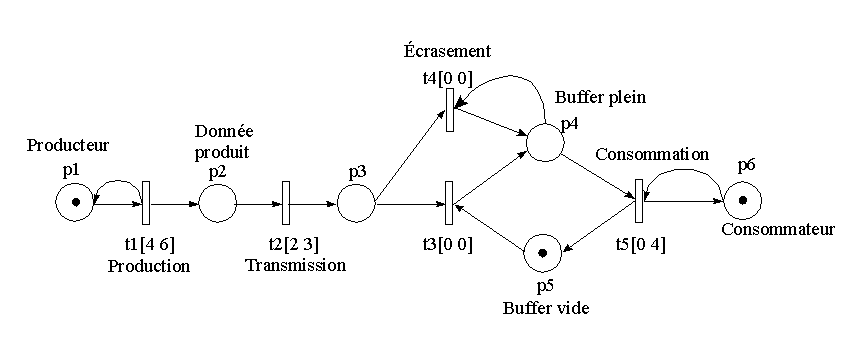
\includegraphics[width=12cm]{figCharles/rdp_exo}}
%\end{figure}

%\end{frame}

%-------------------------------------------------------------------------%
%\begin{frame}
%\frametitle{Réseaux de Petri t-temporels ~2/3}

%Intervalle temporel $I(t_i)=[a_i,b_i]$ : \small {ensemble des
%dates de tir possibles de $t_i$ à partir de sa date de
%sensibilisation.}

%\vspace{-1ex}
%\begin{figure}[h]
%\centerline{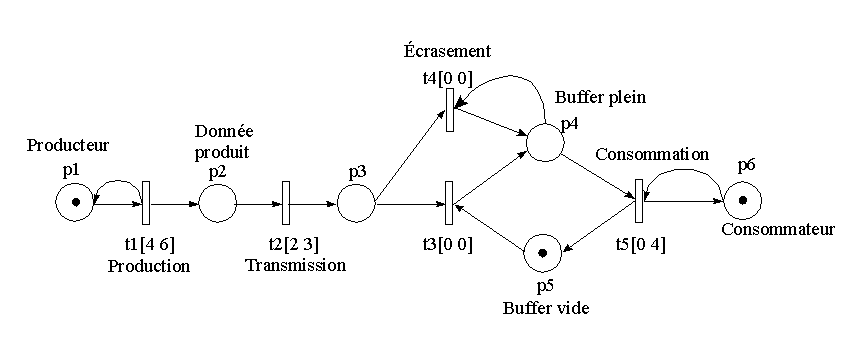
\includegraphics[width=12cm]{figCharles/rdp_exo}}% fig en français
%\end{figure}

%\vspace{-4ex}
%\only{~~~~Les événements à considérer : \small {
%\begin{itemize}
%\item {la date de
%\emph{\textcolor[rgb]{0.00,0.00,1.00}{sensibilisation}} d'une
%transition $t_i$}

%\pause
%\item {la date de \emph{\textcolor[rgb]{0.00,0.00,1.00}{début}} et  la
%date de \emph{\textcolor[rgb]{0.00,0.00,1.00}{fin}} de
%l'intervalle de tir,}

%\pause
%\item {la date de
%\emph{\textcolor[rgb]{0.00,0.00,1.00}{franchissement}} effectif de
%$t_i$.}
%\end{itemize}
%}}

%\end{frame}

%-----Sémantique d'entrelancement-----------------------------------------------%

%\begin{frame}

%\frametitle{Sémantique}

%\begin{columns}
%\column{.05\textwidth}\column{.65\textwidth}

%{\tt \bf Sémantique d'entrelacement :}\\

%\begin{small}
%\vspace{1ex} $\bullet$ ~transitions sensibilisées en parallèle, \\
%mais franchies \textcolor[rgb]{0.00,0.00,1.00}{séquentiellement} \\
%(serveur unique  + durée de franchissement nulle);\\

%\vspace{1ex}

%$\bullet$ ~au lieu $t_1 \| t_2$, on considère \\
%~~~~~~~~~~~$t_1 \, ; \, t_2$ ou $t_2 \, ; \, t_1$.
%\end{small}
%\column{.35\textwidth}
%\centerline{\includegraphics[width=3.5cm]{figCharles/rdp_s_entre}}
%\end{columns}

%\pause
%\begin{columns}

%\column{.35\textwidth}

%\centerline{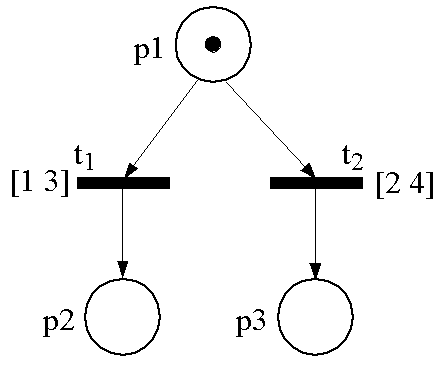
\includegraphics[width=3.5cm]{figCharles/rdp_s_forte}}
%\column{.05\textwidth}\column{.65\textwidth}

%\vspace{2ex}
%{\tt \bf Sémantique forte :}\\

%\vspace{1ex}
%\begin{small}
%$\bullet$ ~si plusieurs transitions franchissables
%$I(t_i)=[a_i,b_i]$: franchir l'une d'elles avant la
%\textcolor[rgb]{0.00,0.00,1.00}{fin} de l'intervalle de tir des
%autres transitions.

%\vspace{1ex}
%\pause
%$\bullet$ ~tir de $t_1$ avant $t_2$ ($b_2=$
%$\textcolor[rgb]{1.00,0.00,0.00}{4}$)
%$\rightarrow$ donc, $t_1 ~[1~3]$.

%\vspace{1ex}
%\pause
%\only<2>{ 
%$\bullet$ ~tir $t_2$ avant $t_1$ ($b_1=$
%$\textcolor[rgb]{1.00,0.00,0.00}{3}$)
%$\rightarrow$ donc, $t_2$ $[2
%\textcolor[rgb]{1.00,0.00,0.00}{~3]}$.%}

%\end{small}



%\end{columns}

%\end{frame}


%------------------
%\subsection{Réseaux de contraintes temporelles}
%\begin{frame}
%\frametitle{Réseaux de contraintes temporelles}

%Représente les contraintes temporelles à un moment donné

%\vspace{1ex}
%\begin{columns}

%\column{.4\textwidth}
%\centerline{\includegraphics[width=3cm]{figCharles/rdp_stn}}

%\column{.3\textwidth}
%\only<1>{\centerline{\includegraphics[width=2.7cm]{figCharles/stn0_nodes}}}
%\only<2>{\centerline{\includegraphics[width=2.7cm]{figCharles/stn0}}}%avec arcs

%\only<3,4>{\centerline{\includegraphics[width=2.7cm]{figCharles/stn1}}}%avec [0,inf)

%\column{.3\textwidth}
%\only<4>{\centerline{\includegraphics[width=2.7cm]{figCharles/stn4}}}

%\end{columns}

%\begin{itemize}
%\item  Ensemble fini de variables : $X$ = \{$x_0$, $x_1$, $x_2$\}
%    \begin{itemize}
%    \item \{$x_1$, $x_2$\} $\backsim$ transitions sensibilisées : $t_1$, $t_2$

%    \item $x_0$ $\backsim$ date \textcolor[rgb]{0.00,0.00,1.00}{sensibilisation}
%    de $t_1$ et $t_2$ (arrivée de jetons)
%    \end{itemize}

%  \only<2,3,4>{\item Ensemble fini de contraintes $C$ :
%      \begin{itemize}
%      \item ($x_0$, $x_1$) = [1~2]; ($x_0$, $x_2$) = [3~4] $\backsim$
%      \textcolor[rgb]{0.00,0.00,1.00}{intervalle de tir} de $t_1$, $t_2$
%      \only<3,4>{\item ($x_1$, $x_2$) = [0~$\infty$) $\backsim$
%      franchir $t_2$ après $t_1$}
%      \end{itemize}}%only item

%\only<4>{\item Algorithme de Floyd-Warshall  (plus court chemin):
%STN \emph{minimal}.\\
% {\small $\blacktriangleright$  \textcolor[rgb]{0.00,0.00,1.00}{franchissement} de la transition $t_2$ :
% [1~3] après $t_1$}}
%\end{itemize}

%\end{frame}

%\begin{frame}
%\frametitle{RdP : graphe de marquage}

%\begin{columns}
%\column{.45\textwidth}

%\centerline{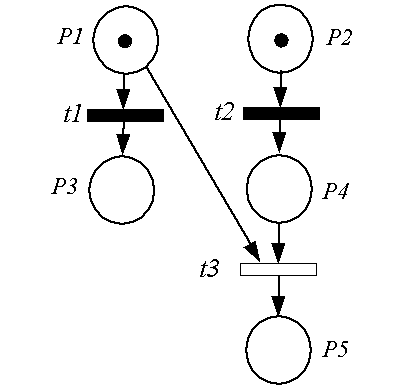
\includegraphics[height=4cm]{figCharles/rdp_sanst}} \vspace{1ex}
%\centerline{Réseau de Petri atemporel}

%\column{.05\textwidth} $\stackrel{analyse}{\longrightarrow}$

%\column{.50\textwidth}

%\centerline{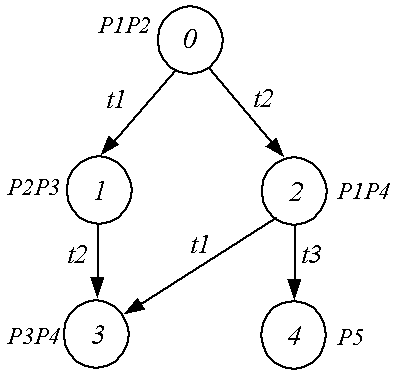
\includegraphics[height=4cm]{figCharles/graph_m}} \vspace{1ex}
%\centerline{Graphe de marquage}

%\end{columns}
%\end{frame}
%---------------------------------------------------------------------------------%

%\begin{frame}
%\frametitle{RdP temporel : graphe de classes}

%\begin{columns}
%\column{.3\textwidth}
%\centerline{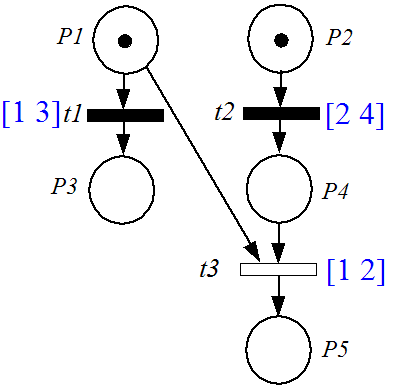
\includegraphics[height=4cm]{figCharles/rdp_temps_ch}}
%\vspace{2ex} \centerline{Réseau de Petri
%\textcolor[rgb]{0.00,0.00,1.00}{Temporel}}

%\column{.7\textwidth}
%\begin{itemize}
%\item Prise en compte du temps :
%\begin{itemize}
%\item Nombre infini d'états (marquage + temps) \item Nombre infini
%de séquences
%\end{itemize}

%\item Il faut :
%\begin{itemize}
%\item Regrouper les états en un nombre fini de classes : 
%\emph{oublier} une partie du passé.

%\item Classe ${\cal C}$ : donne les  intervalles de tir et les contraintes
%temporelles que doivent vérifier les
%transitions vis-à-vis des franchissements
%passés.
%\end{itemize}
%\end{itemize}

%\end{columns}
%\end{frame}

%\begin{frame}
%\frametitle{Graphe de classes}

%\begin{columns}
%\column{.4\textwidth}
%\centerline{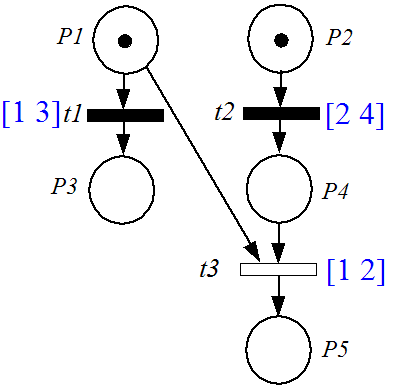
\includegraphics[height=4cm]{figCharles/rdp_temps_ch}}
%\vspace{2ex} \centerline{Réseau de Petri
%\textcolor[rgb]{0.00,0.00,1.00}{Temporel}}

%\column{.6\textwidth}

%\textbf{État}: \{$M$, $I(t)$\}
%\begin{itemize}
%  \item $M$: Marquage
%  \item $I(t)$: Fonction temporelle
%\end{itemize}


%\vspace{2ex} \textbf{Classe d'états}:

%composée par tous les états que sont atteignables par une séquence
%de tir.

%\vspace{2ex} Plusieurs définitions de classe, selon le type de
%propriétés à prouver :
%\begin{enumerate}
%  \item mode Linear,  {\footnotesize (B.Berthomieu)} % (LTL properties)%
%  \item mode Arborescent,  {\footnotesize (B.Berthomieu)} % (CTL properties)%
%    \item mode C,  {\footnotesize (J. Cardoso, R. Valette)} 
%\end{enumerate}

%\end{columns}
%\end{frame}

%\begin{frame}
%\frametitle{Graphe de classes mode linéaire}% {\footnotesize (B.Berthomieu)}

%\begin{columns}
%\column{.45\textwidth}

%\only<1,2>{\centerline{\includegraphics[height=4cm]{figCharles/rdp_temps_ch}}
%\vspace{1ex} \centerline{Réseau de Petri
%\textcolor[rgb]{0.00,0.00,1.00}{Temporel}} }

%----------
%\only<3>{\centerline{\includegraphics[height=4cm]{figCharles/rdp_c1}}
%\vspace{1ex} \centerline{Réseau de Petri
%\textcolor[rgb]{0.00,0.00,1.00}{Temporel}}  \vspace{1ex} }

%----------
%\only<4,5>{\centerline{\includegraphics[height=4cm]{figCharles/rdp_c2}}
%\vspace{1ex} \centerline{Réseau de Petri
%\textcolor[rgb]{0.00,0.00,1.00}{Temporel}}  \vspace{1ex} }

%----------
%\only<6>{\centerline{\includegraphics[height=4cm]{figCharles/rdp_c3}}
%\vspace{1ex} \centerline{Réseau de Petri
%\textcolor[rgb]{0.00,0.00,1.00}{Temporel}}  \vspace{1ex} }

%\column{.55\textwidth} 

%-------------
%\only<1>{\centerline{\includegraphics[width=5cm]{figCharles/horloge_che_a}}

%\centerline{\includegraphics[height=4.2cm]{figCharles/graph_wd}}

%}

%-------------
%\only<2>{\centerline{\includegraphics[width=5cm]{figCharles/horloge_che_a}}

%\centerline{\includegraphics[height=4.2cm]{figCharles/graph_wd}}

%\centerline{\textcolor[rgb]{1.00,0.00,0.00}{Tous ces états
%sont-ils atteignables!?}}}

%----------
%\only<3>{\centerline{\includegraphics[width=5cm]{figCharles/horloge_che1_a}}
%\centerline{\includegraphics[height=3.5cm]{figCharles/graph_wd2}}

%\centerline{Si $t2$ est franchie au temps
%\textcolor[rgb]{1.00,0.00,0.00}{3}}$\ldots$  $t3$ est-elle encore
%franchissable?}

%----------
%\only<4>{\centerline{\includegraphics[width=5cm]{figCharles/horloge_che2_a}}

%\centerline{\includegraphics[height=3.5cm]{figCharles/graph_wd2}}

%\centerline{Si $t2$ est franchie au temps
%\textcolor[rgb]{1.00,0.00,0.00}{3}}$\ldots$  $t3$ est-elle encore
%franchissable?}
%----------
%\only<5>{\centerline{\includegraphics[width=5cm]{figCharles/horloge_che3_a}}

%\centerline{\includegraphics[height=3.5cm]{figCharles/graph_wd2}}

%\centerline{Si $t2$ est franchie au temps
%\textcolor[rgb]{1.00,0.00,0.00}{3}}$\ldots$  $t3$ est-elle encore
%franchissable?}
%----------
%----------
%\only<6>{\centerline{\includegraphics[width=5cm]{figCharles/horloge_che4_a}}

%\centerline{\includegraphics[height=3.5cm]{figCharles/graph_wd2}}

%\centerline{Si $t2$ est franchie au temps
%\textcolor[rgb]{1.00,0.00,0.00}{3}}$\ldots$  $t3$ est-elle encore
%franchissable?
% ~~~~\textcolor[rgb]{1.00,0.00,0.00}{\textbf{Non!}}%d
% }

%\end{columns}
%\end{frame}


%-------------------------------------------------------------------%

%\begin{frame}
%\frametitle{Graphe de classes mode arborescent}% {\footnotesize (B.Berthomieu)}
%\begin{columns}

%\column{.43\textwidth}
%%----------
%\centerline{\includegraphics[height=4cm]{figCharles/graph_wd}} \vspace{1ex}
%Mode linéaire

%\vspace{-1ex}
%\begin{itemize}
%  \item Problème branchement~:  distinguer les états dans le futur.
%\end{itemize}
%\vspace{2ex}
%%----------
%\column{.07\textwidth}
%\centerline{\includegraphics[width=2cm]{figCharles/passage_wa}}

%%----------
%%right column
%\column{.50\textwidth}
%\centerline{\includegraphics[height=4cm]{figCharles/graph_a}} \vspace{1ex}
%~~Mode arborescent
%
%\vspace{-1ex}
%\begin{itemize}
%  \item Problème branchement : résolu
%  \item Mais encore problème de chemin : distinguer les états dans le passé.
%\end{itemize}
%
%\end{columns}
%
%\end{frame}
%
%%------------------------------------------------------------------------------%
%\begin{frame}
%\frametitle{Graphe de classes mode C}%Proposition : g
%
%\begin{columns}
%% left column
%\column{.49\textwidth}
%\centerline{\includegraphics[height=4cm]{figCharles/graph_a}} \vspace{1ex}
%~~Mode arborescent
%
%\vspace{-1ex}
%\begin{itemize}
%  \item Problème branchement : résolu
%  \item Mais encore problème de chemin : distinguer les états dans le passé.
%\end{itemize}
%
%%middle column
%\column{.04\textwidth}
%%\centerline{\includegraphics[width=1.8cm]{passage_ac}}
%.
%
%% right column
%\column{.46\textwidth}
%\centerline{\includegraphics[height=4cm]{figCharles/graph_c}} \vspace{1ex}
%%\centerline{Classes Graph's proposal }
%\centerline{Mode C}%Notre approche: 
%
%\vspace{-1ex}
%\begin{itemize}
%  \item Problème branchement : résolu
%  \item Problème de chemin : résolu
%\end{itemize}
%\vspace{3ex}
%
%\end{columns}
%\end{frame}

% \begin{frame}
% \frametitle{Calcul du graphe de classes mode linéaire}
% 
% Graphe de classes :
% \begin{itemize}
%\item noeuds (classes $C_i$) :
%\begin{itemize}
%\item états avec le même marquage,
%\item domaine temporel (union des domaines temporels des états) :
%\begin{itemize}
%\item  intervalle de temps des transitions sensibilisées
%\item  contraintes temporelles entre couples de transitions sensibilisées (mémoire temporelle depuis la classe où elles étaient sensibilisées) ;
%\end{itemize}


%\end{itemize}
%\item arcs $(C_i,C_j)$ : intervalle de tir de $t$, avec $C_i \stackrel{t}{\rightarrow}C_j$
%\end{itemize}
%\includegraphics[height=3cm]{figCharles/rdp_temps_ch}
% \end{frame}

% \begin{frame}
% \frametitle{Protocole unidirectionnel de transfert de données}

%\vspace{-.2cm}
%\centerline{\includegraphics[width=10cm]{figCharles/rdp_exo}}

%~~RdP  {\color{blue}sans} le temps :\\
 
% \vspace{.2cm} 
%\begin{columns}
%\column{.5\textwidth}
%{\scriptsize
%\hspace{.5cm}Graphe de marquage non borné\\

%\vspace{.2cm} 
%\hspace{.5cm}path from 0 to 1 increases marking\\
%\hspace{.5cm}0 : p1 p5 p6\\
%\hspace{.5cm}1 : p1 p2 p5 p6\\

%\vspace{.2cm} 
%\hspace{.5cm}REACHABILITY GRAPH:\\
%\hspace{.5cm}0 -$>$ t1/1\\
%\hspace{.5cm}1 -$>$ t1/?, t2/?
%~\\

%\vspace{.4cm} 
%}

% \column{.5\textwidth}
% {\scriptsize
%  Graphe de couverture\\
%  \includegraphics[width=5cm]{./figSH/ExIfac_gCk}\\
%  CLASSES:\\

%0 : p1 p5 p6\\
%1 : p1 p2*w p5 p6\\
%2 : p1 p2*w p3*w p5 p6\\
%3 : p1 p2*w p3*w p4 p6\\

%}

% \end{columns}
% \end{frame} 
%  \begin{frame}
% \frametitle{Protocole unidirectionnel de transfert de données}

%\vspace{-.2cm}
%\centerline{\includegraphics[width=10cm]{figCharles/rdp_exo}}
%\begin{columns}
% \column{.5\textwidth}
%{\scriptsize Les classes (marquage + domaine temporel)} : \\
% \includegraphics[width=4.4cm]{./figSH/clas1}\\
%\includegraphics[width=6cm]{./figSH/cla2}\\

%\column{.48\textwidth}
% \includegraphics[width=5.3cm]{figCharles/w}

% \end{columns}
% {\scriptsize Intervalle de tir $D^j(t_i)$ de $t_i$ à partir de $C_j$ :\\
%$D^0(t_1)=[4,6]$, $D^1(t_2)=[2,3]$, $D^2(t_3)=[0,0]$, $D^4(t_2)=[2.3]$, $D^4(t_5)=[0,3]$, $D^5(t_4)=D^5(t_5)=[0,0]$, $D^3(t_1)=[1,4]$, $D^3(t_5)=[0,4]$, $D^6(t_2)=[1,3]$, $D^7(t_1)=[0,4]$ }% fin script
% \end{frame} 

\end{document}
